% TODO:
%   - Refs to sections check if truly explained there
%   - Cleanup of text
% ----------  
% Questions:
%   -

% TODO: mentionen dat geen systematic review a la standaarden zoals arnau maar wel goed en ook zeggen Zotero

% NOTE: Uncomment this if the use of parts is desired
\part{Understanding Brain-computer interfaces}


% NOTE: In a new chapter, reset the GLS to once again use the full version in the first occurrence
\glsresetall

\chapter{Brain-Computer interfaces}
\label{ch:bci}

% ---------------------------------------------- 
% INTRODUCTION
% ---------------------------------------------- 
\section{Introduction to this chapter}
\label{sec:bci_introduction}
% NOTE: "Introduction" exists in each chapter and gives short intro to chapter + what can be expected in chapter

\Glspl{bci} are systems, consisting of hardware and software, that aim to read or even stimulate a user's brain signals for a wide variety of applications.
Whilst many of these applications for \glspl{bci} revolve around providing novel interaction methods for computer applications, they are capable of fulfilling more general tasks as well.
Because of this, \glspl{bci} are also referred to as \glspl{bmi} and can be seen as a special type of the more general \glspl{hmi} and \gls{bc} systems.
A well-known Professor in this field is Jonathan R. Wolpaw who was also the guest editor for the first international meeting devoted to \gls{bci} research and development as part of the IEEE conference on Rehabilitation Engineering.
During that meeting, a first formal definition for \glspl{bci} was given:

\setlength{\epigraphwidth}{0.9\textwidth}
\epigraph{A brain-computer interface is a communication system that does not depend on the brain’s normal output pathways of peripheral nerves and muscles.}{\textit{\citet{first_bci_meeting}}}

Since then, Jonathan R. Wolpaw has (co-)authored a lot of influential papers in the field of \glspl{bci} \citep{bci_rehabilitation, bci_in_medicine, first_bci_meeting} and created a great introductory textbook to the field \citep{bci_book}.
As a board-certified neurologist, Wolpaw's work is often centred around applications in a more medical setting rather than a commercial one. In this medical setting, his opinion on what defines a \textit{perfect} \gls{bci} is often strived for and can be summarized as follows:

\setlength{\epigraphwidth}{0.9\textwidth}
\epigraph{The perfect [medical] \gls{bci} is a safe and affordable system which works all the time, does not require the permanent assistance of a technician or a scientist, restores communication at “normal” speed, is aesthetically acceptable, is reliable and, for the same function, does not require more concentration for a patient user than what it does for an able-bodied person.}{\textit{\citet{bci_book, cheap_bci_feasibility}}}


One of the things this thesis aims to study is how far \glspl{bci} have come concerning this definition of a perfect \gls{bci}.
It is noted that the term communication in these definitions simply depicts the exchange of information rather than specific human communication such as speech. For example, a computer mouse could be seen as a communication device that exchanges information about the user's intent to the computer.
Many of these properties for a perfect medical \gls{bci} system would also be beneficial for commercial \gls{bci} systems.

Especially the commercial interest in \glspl{bci} has seen a recent spike, through multiple big-tech companies such as Meta (formerly known as Facebook), Valve (a major gaming company) and Neuralink (an Elon Musk company) showing interest in the field \citep{facebook_bci_blog, bci_valve, neuralink_whitepaper}.
This has given rise to the public interest for potential life-improving \gls{bci} applications as well as some public outrage on more ethical aspects that challenges these systems. 

This first part of the thesis aims to provide all required background information needed for understanding \glspl{bci}.
The remainder of this chapter further introduces the main rationale behind \glspl{bci} research by discussing the rise in popularity of both medical and commercial \glspl{bci}, some practical examples of \gls{bci} systems that have been developed and some of the opportunities and obstacles in the field. The chapter ends with a note on some of the ethical challenges for \gls{bci} systems and a discussion of the proposed system for this thesis.
Chapter \ref{ch:biomedical_signals} gives more depth on the origins and measurability of brain signals while Chapter \ref{ch:processing_signals} addresses the techniques and technologies needed to process brain-signals and take actions based on their interpretation. 
As research on \glspl{bci} is highly multidisciplinary, entering the field as a computer scientist can be rather intimidating due to the steep learning curve of the ideas, technologies, challenges and terminology used in such research.
To lower this initial learning curve, these first three chapters aim to introduce the most important concepts in an easy-to-understand manner for a typical computer scientist student with some \gls{ai} background.
These first chapters follow no specific systematic review procedure.
However, special attention was payed to favor papers from reputable sources, such as famous authors in the field (i.e. Jonathan R. Wolpaw).
A focus was also put on articles which have been influential based on both the amount of times the work itself is cited in other articles and the performance of these other articles citing the original article.
The latter was determined by using the connected papers tool\footnote{\url{https://www.connectedpapers.com/}}.

The interested reader is also referred to the great introductory book on \glspl{bci} by \citet{bci_book} and the review article by \citet{bci_review} when more introductory insight is desired.
Whilst these resources have dated a little and state-of-the-art has changed since then, the main ideas discussed in them remain unchanged.
A more recent, systematic review article by \citet{bci_review_arnau} focuses on current \gls{dl} techniques for use with \glspl{bci} among other \gls{bc} systems.


% ---------------------------------------------- 
% GAINING POPULARITY
% ---------------------------------------------- 

\section{Growing scientific and commercial interest in BCIs}
\label{sec:bci_gaining_popularity}

With brain signal measuring modalities such as \gls{eeg} being over 100 years old, the idea of using those brain signals for a wide variety of use cases has been explored for many decades \citep{human_eeg_discovery, first_eeg, bci_history}.
With feasibility studies of using \glspl{bci} already existing in the 1970s \citep[for example by][]{early_bci} showing that most of the ideas explored today are not new, a clear spike in both scientific and commercial interest can be seen after the 2000s.
It is no coincidence that the first international meeting devoted to \gls{bci} research and development as part of the IEEE conference on Rehabilitation Engineering discussed in Section \ref{sec:bci_introduction} was also from this period.

This rise in popularity can be explained by several events.
Perhaps most importantly is the improvement of both brain signal measuring equipment and computational processing equipment in both efficiency, accuracy and portability.
Recent improvements in \gls{ml} and \gls{dl} after some \gls{ai} winters between the 1970s and the 1990s are bound to also have played an important role.
The interest of big tech companies such as Neuralink, Meta and Valve have also introduced unseen amounts of funds further accelerating \gls{bci} research.

This section focuses on discussing these most important contributing factors to the new rise of interest in \gls{bci} research.
These factors are discussed in an arbitrary order, as most of them have influenced each other and it is hard to name a singular reason that explains this recent rise in interest.
For a more in-depth overview of the rich history that \gls{bci} research has, the reader is referred to the work by \citet{bci_history}.

% - - - - - - - - - -
% big tech
% - - - - - - - - - -

\subsection{BCIs have gained big-tech interest and funds}
\label{subsec:bci_gaining_popularity_big_tech}

Big tech has been catching on with the possibilities \glspl{bci} bring, and the amount of money they can earn from it.
Although profitability is an important factor in most medical applications as well, the focus of medical applications lies on improving the life of a patient, whilst the focus of commercial applications can differ greatly.
Since commercial \glspl{bci} are still in their early stages and the idea of constantly wearing a brain-signal recording headset has not been accepted by the wide public yet, many commercially oriented companies start with products that are a cross between medical and commercial applications.

Most noteworthy of these more commercially oriented companies is Neuralink, an Elon Musk company.
Neuralink's initial white paper discusses its aim to create a scalable high-bandwidth \gls{bci} system, focusing on its mechanical achievements \citep{neuralink_whitepaper}.
These mechanical achievements are rather impressive, with state-of-the-art robot surgery inserting ultra-thin sensors directly into the skull allowing for a sleek and visually pleasing package that is mostly hidden from the human eye.
Comparing this to non-invasive methods of recording brain signals, which are methods that don't require inserting machinery into the human body, the signal quality is also expected to be far greater.
However, an invasive approach currently introduces added health risks and more ethical challenges making non-invasive methods often more suited for general use \citep{neuralink_ethics, neuralink_ethics2, bci_review_arnau}.
Since the publication of the Neuralink white paper, the company has held live demos of their \gls{bci} implanted directly into the skulls of animals such as pigs and monkeys.
A video by Neuralink of a monkey playing pong using brain signals as input\footnote{\url{https://youtu.be/rsCul1sp4hQ}} has gathered over 6 million views on YouTube already.
Combined with many news articles, the kind of exposure that Neuralink has gotten is unseen compared to the regular exposure of literature in the field.
This can be questioned, as earlier work by \citet{bci_monkey_arms} demonstrated monkeys taking control over two avatar arms simultaneously, a task that is arguably even harder to accomplish than simply playing pong.
Adding to this, the experiment by \citet{bci_monkey_arms} has an appropriate peer-reviewed paper backing it whilst Neuralink among other commercially oriented companies in the field often lack scientific backing for the claims they make.
Thus, the scientific value of these more commercial demos and applications can be argued for, but the funds for research introduced by these companies and the exposure to the field have accelerated research in the field and helped popularize the field.
Adding to this, the proposed system by Neuralink is one of the most aesthetically pleasing compared to alternative invasive or non-invasive systems on the market, which is one of the properties of Wolpaw's perfect \gls{bci} system given in Section \ref{sec:bci_introduction}.

Besides Neuralink, companies like Meta, Valve, Neurable, InteraXon and many more are exploring the commercial possibilities of \glspl{bci} as well.
Some of the companies do this through direct internal research whilst others might provide funds for external projects \citep{facebook_bci_keyboard, valve_bci_interest, neurable_white_paper, interaxon_tests}.
There seem to be two main focuses of the technology in the commercial space.
Either using the new interaction method to perform work more efficiently or using it for recreational purposes.

% | | | | | | | | | | | | |

\subsubsection{Using BCIs to boost work efficiency}
\label{subsubsec:bci_gaining_popularity_big_tech_efficiency}

Meta, formerly known as Facebook, has been playing with the idea of \glspl{bci} for quite a while but has been relatively quiet about it publicly.
In 2021, Meta publicly announced it had provided funds for research on the use of a \gls{bci}-system to restore speech functionalities for people suffering from anarthria \citep{facebook_bci_keyboard, facebook_bci_blog}.
The system by \citet{facebook_bci_keyboard} achieved an average of 15 words per minute, decoded with a median error of 25\%.
Whilst this might not sound impressive, anarthria is a disease which causes patients to not be able to articulate speech at all due to lost control of the muscles required for making sounds.
Adding to this, people suffering from anarthria often suffer from other lost muscle control as well, making alternatives such as keyboard typing or writing impossible.
Taking this into account, these results should be seen as very impressive and such a system can be life-changing for certain patients.
Whilst the system by \citet{facebook_bci_keyboard} was invasive just like Neuralink's system, it was far from visually pleasing.
The patient was fixed in a chair and physically connected to a bulky processing unit in the form of a small server rack, which makes the system non-mobile and makes the user stand out if it were to be used in the real world where discreteness is often desired.

The system by \citet{facebook_bci_keyboard} is an example of one that is backed by the funds that big-tech companies have and which is mainly focused on medical applications whilst the final intention of the funding company is most likely of commercial nature.
Indeed, it is not hard to imagine the commercial interest of Meta in developing a more general \textit{virtual keyboard} to enable fast \textit{thought to speech} or \textit{thought to text} applications usable by the masses.
In fact, during the F8 conference \citep{fb_building8} a couple of years before the paper by \citet{facebook_bci_keyboard}, Meta stated the following:


\setlength{\epigraphwidth}{0.9\textwidth}
\epigraph{Specifically, we have a goal of creating a silent speech system capable of typing 100 words per minute straight from your brain – that’s five times faster than you can type on a smartphone today.}{\textit{\citet{fb_building8}}}


Such a virtual keyboard could replace certain speech-to-text applications already broadly used for commercial purposes.
In the same blog post by \citet{facebook_bci_blog} discussing the funding for the project by \citet{facebook_bci_keyboard}, it is also mentioned that Meta has interest in using \glspl{bci} for high-bandwidth interactions in AR/VR.
However, Meta has been subject to multiple privacy concerns lately \citep{facebook_drama1, facebook_drama2}.
The company's reputation has been damaged from this which doesn't help in selling the concept of them having a \gls{bci} which allows them to read the brain activity of the users.
This could explain why they have recently started to shift their focus from \glspl{bci} towards muscle-based interfaces using \gls{emg} \citep{facebook_bci_blog}.

A recent example of a \gls{bci} being used to boost work efficiency is covered by \citet{bci_nude_detection}.
He discusses how Chinese researchers have been working on a non-invasive and portable system that aims to detect if a user is watching pornographic content through brain signals.
When presenting fifteen male participants aged between 20 and 25 with erotic content and regular content, an accuracy of over 80\% was obtained for determining whether the user was watching erotic content or not.
Such a system should aid in China's content regularisation which often bans such erotic content on their domestic social-media platforms.
Current systems rely on manual evaluation by a reviewer for removing or keeping content that is flagged as inappropriate by either the community or an algorithm. 
Further automating this task through a brain-controlled system could boost the efficiency of this process significantly.


% | | | | | | | | | | | | |

\subsubsection{Using BCIs for recreational use}
\label{subsubsec:bci_gaining_popularity_big_tech_recreational}

Whilst some promising results have been obtained when using \glspl{bci} in commercial settings to boost work efficiency, many of the systems still lack the desired performance to become truly viable. 
And thus, the most prominent type of commercial \glspl{bci} are those focusing on recreational use.
In this regard, the headsets by InteraXon, produced under the Muse brand, are one of the earliest examples, with their first version being released in 2014.
The first iteration of this product was advertised as a meditation aid.
This headset relies on measuring Theta waves in the brain, which are lower frequency waves that suggest a user is meditating.
Section \ref{subsec:biomedical_signals_brain_signals_brain_waves} talks about these brain wave frequencies in more detail.
The actual accuracy and usefulness of these types of systems are debated, as discussed by \citet{interaxon_tests}.
More recently, a newer version of the InteraXon headset came to market, named Muse 2, which also aids in sleep monitoring.
This relies on detecting Delta waves among other patterns to determine the sleep quality of a user.
Like before, this accuracy and usefulness can be argued for.
A similar commercial product for sleep tracking is available from the company Dreem, under the name Dreem 2.
Dreem has received more funding, as can be seen in Figure \ref{fig:bci_money}, but InteraXon, the company behind the Muse headset, has arguably contributed more to the field.
Not only was it one of the first commercial \glspl{bci} that gained media attention, but the company also plays an important role in the commercialisation of \glspl{bci} as their headsets are cheap, non-invasive and visually pleasing whilst also being widely available. 
Adding to this, these headsets have pretty good supporting libraries in Python among other programming languages that allow developers to use these headsets for other purposes as well.
Besides InteraXon, some other companies that specialize in providing commercially usable brain-signal recording headsets exist, as will be further discussed in Section \ref{subsec:biomedical_signals_measuring_equipment}.

Perhaps the most promising short-term commercial use of \glspl{bci} is in combination with \gls{vr} and \gls{ar}.
Besides Meta's interest in this region, as discussed earlier in this section, Valve has also said it is actively researching how to use \glspl{bci} as a novel interaction system in \gls{vr} games \citep{valve_bci_interest}.
Valve is the company behind Steam, one of the world's largest game marketplaces and they are specialized in creating games and gaming hardware as well.
To achieve the goals of this project code-named \textit{Galea}, Valve is working together with OpenBCI, a well-respected company in the \gls{bci} research field that has provided open-source hardware and software for use in \gls{bci} systems.
Tobii, a company that specializes in eye-tracking software, is also working on project Galea.
With a final goal of creating an open-source \gls{bci} that can be used in gaming, the anticipation for the headset has been high.
However, just as with deadlines from other companies such as Meta and Neuralink, the project has been postponed multiple times.
This is not surprising as the promises of what a \gls{bci} can do are near endless and initial trials often offer promising results but going to a final product has been proven to be incredibly hard due to several open issues \citep{bci_review_arnau}.

A final stream of money that is important to mention, is coming from militaries around the globe.
The U.S. military among others is known to invest a lot of money in any form of innovation, especially related to devices and technologies that can give them a strategic edge when fighting in a war \citep[with examples of funds for AI research in][]{military_ai_money, military_ai_money_eu}.
Whilst most of this information is classified, it is known that the U.S. Department of Defense and others have shown interest in a wide variety of applications using \glspl{bci} \citep{bci_military}.
Whilst one can only guess what these government organisations are developing, it is likely that over time these applications might become public knowledge and aid the research field of \glspl{bci} in creating even better systems.
\Citet{us_military_bci} discusses the U.S. militaries interest in \glspl{bci} further.

% | | | | | | | | | | | | |

\subsubsection{Summary of big-tech using BCIs for commercial applications}
\label{subsubsec:bci_gaining_popularity_big_tech_summary}

To summarize, there have been a lot of big companies showing interest in commercial \gls{bci} applications in the past few years.
Some might contribute directly to the field by funding scientific research, which is often still focused on medical applications but whose results can show potential for certain commercial applications \citep{facebook_bci_blog, facebook_bci_keyboard, neuralink_whitepaper}.
On the other hand, some companies are working on commercial products internally, mostly for improving work efficiency \citep{fb_building8, bci_nude_detection} or for recreational use \citep[Muse and InteraXon headband,][]{valve_bci_interest}.
These commercial products have yet to see truly successful examples, as they are either questionable in delivering what they promise \citep{interaxon_tests}, experience delayed deadlines or are even cancelled in their entirety.
Nonetheless, these companies focusing on commercial applications often have high amounts of funding and a focus on the \gls{ux} of \glspl{bci} which could help accelerate research in the field and make \gls{bci} systems more visually pleasing and accepted by the broader public.
In this way, they also contribute to Wolpaw's vision of a perfect \gls{bci} system as discussed in Section \ref{sec:bci_introduction}.

Figure \ref{fig:bci_money} shows the funding of \gls{bci}-related companies founded after 2010 as a rough indication of how much money is spent on start-up companies in the field.
Interestingly, from the companies Neurable, Muse and Neuralink mentioned in this thesis, the funding amount is in proportion to the overall popularity of that company to the wider public, although this is by no means a proven relation.
It also shows that whilst academic research on \glspl{bci} doesn't require huge funding, with open-source datasets and relatively cheap hardware available as is further discussed in Section \ref{subsec:bci_gaining_popularity_improved_data_processing}, \ref{subsec:biomedical_signals_measuring_equipment}, and \ref{subsec:processing_signals_alternative_pipelines_using_existing_data}, creating an effective commercial product can become an expensive affaire rather quickly.

\begin{figure}[ht]
    \centering
    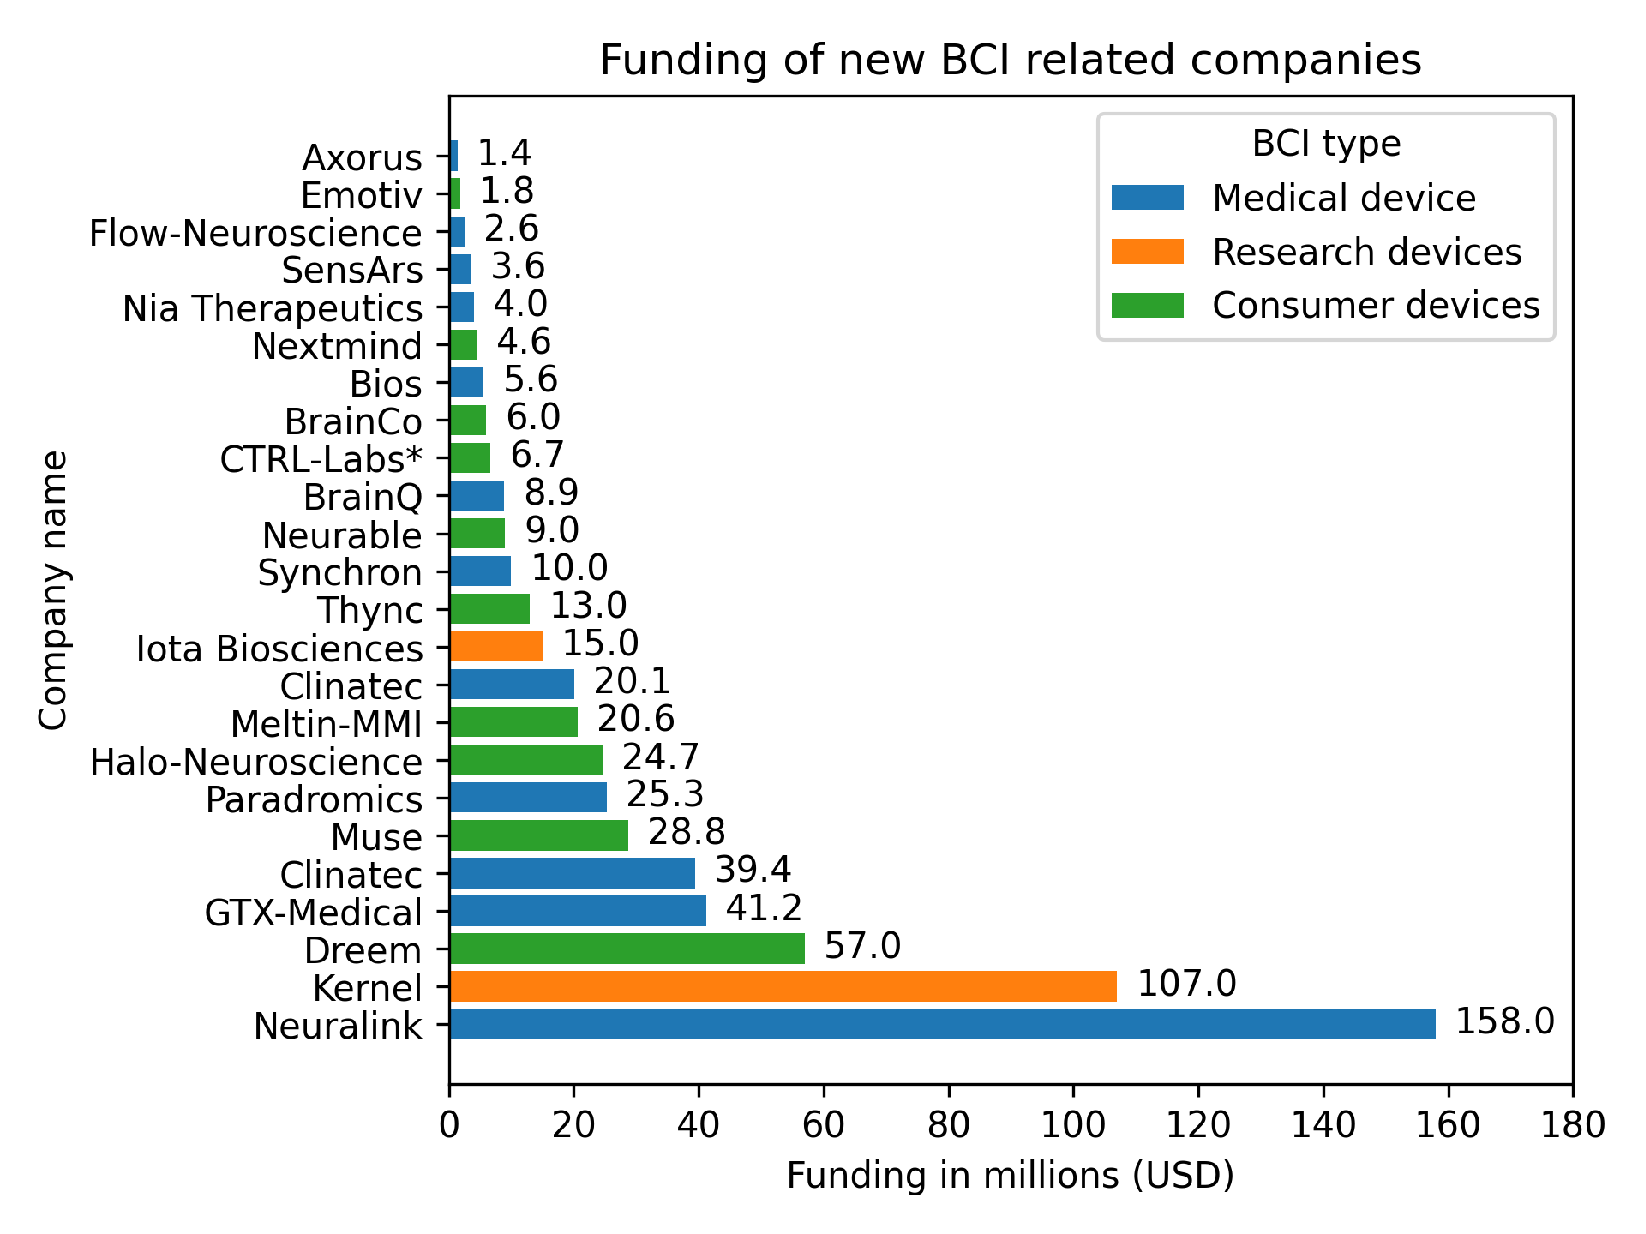
\includegraphics[width=\linewidth]{../images/introduction/funding.pdf}
    \captionsetup{width=0.9\linewidth}
    \captionsetup{justification=centering}
    \caption{Funding of newer \gls{bci} related companies depicted in millions (USD).\\Figure based on data by \citet{bci_money} from 2019. It is noted this data is limited to companies that were created after 2010 where funding information is made available.}
    \label{fig:bci_money}
\end{figure}

% - - - - - - - - - -
% improved hardware
% - - - - - - - - - -


\subsection{Improved brain-signal measuring facilities}
\label{subsec:bci_gaining_popularity_better_measuring}

\glsreset{bci}
\glsreset{hmi}
\glsreset{ux}

As \glspl{bci} are a type of \gls{hmi} relying solely on brain signals to operate, the measuring facilities for acquiring data of those brain signals have a direct impact on the capability of those systems.

Most \glspl{bci} rely on non-invasive measuring equipment that uses \gls{eeg} as a source of data and this paper will focus mainly on such measuring equipment as well.
Chapter \ref{ch:biomedical_signals} explains in greater detail what \gls{eeg} and some of its alternatives are, the equipment used for acquiring brain-signal data and more.
For this introduction, it suffices to know that non-invasive \gls{eeg} measuring equipment measures the electrical potential difference, often in \gls{mv}, between electrodes placed on the scalp.

Following Wolpaw's definition for a perfect \gls{bci} given in Section \ref{sec:bci_introduction}, the recording hardware should ideally be aesthetically acceptable and shouldn't require the assistance of a professional to install.
In recent years, new developments in this hardware have made meeting these criteria more plausible, which are adressed in this section.

% | | | | | | | | | | | | |

\subsubsection{Hardware improvements in non-invasive EEG measuring equipment}
\label{subsubsec:bci_gaining_popularity_better_measuring_hardware}

Three major hardware distinction made between the electrodes used in non-invasive \gls{eeg} measuring equipment is whether they are wet or dry electrodes, whether they are active or passive electrodes and whether communication to the processing unit happens wirelessly or not.
When considering Wolpaw's definition of a perfect \gls{bci} described in Section \ref{sec:bci_introduction}, dry-electrodes with passive amplification that connect wirelessly to the processing unit would be ideal.
However, when looking at data quality, a wired wet-electrode with active amplification is best.
Luckily, recent advancements have made these differences in data quality more acceptable, as will shortly be discussed in what follows.

Wet \gls{eeg} electrodes are electrodes which require an electrolytic gel to be applied between the electrode and the scalp.
This gel functions as a conductor and, as discussed further in Section \ref{subsec:biomedical_signals_measuring_equipment}, currently allows wet electrodes to have better data quality compared to dry electrodes \citep{wet_vs_dry, dry_electrode_status, wet_dry_comparison_experiment}.
However, wet electrodes require the assistance of a professional to correctly apply the gel which leaves behind traces after use.
Adding to this, the electrolytic gel could also cause allergic effects for the user. Due to the viscosity of the electrolytic gel changing over time, artefacts in measurements may also appear \citep{dry_electrode_status}.
These are unwanted properties and conflict with Wolpaw's vision of a perfect \gls{bci}.
The medical-grade \gls{eeg} equipment shown in Figure \ref{fig:example_eeg_measuring_devices_medical_bulky} uses wet electrodes with an electrode cap.

Advancements in dry electrodes are making the gap with wet electrodes smaller and smaller \citep{wet_vs_dry, dry_electrode_status, wet_dry_comparison_experiment}.
These dry electrodes don't require the use of an electrolytic gel and given the use of an appropriate headset can be installed on the scalp without the assistance of a professional. 
Both of these properties are in favour of Wolpaw's properties for a perfect \gls{bci}.
The main reason dry-electrodes are becoming more viable to be used in real-life environments is due to improvements in active electrode technology \citep{wet_vs_dry}.
A relatively bulky setup of these dry electrodes with active amplification is shown in Figure \ref{fig:example_eeg_measuring_devices_commercial_clean}.

Active electrodes are electrodes which do more than just forwarding their measured voltage fluctuation to the main controller board whilst passive electrodes do just that.
This is often necessary since the measured signal is of such low strength that even a short distance cable from the electrode to the main board can cause a lot of noise due to electromagnetic interference \citep{active_electrode_explained}.
To reduce this noise, a preamplifier is used which additionally amplifies the signal before transmission over the wire as opposed to only being amplified in the main controller board.
This makes the final system less compact and more expensive but is often required in anything but lab environments, especially for wireless dry electrodes, as further discussed by \citet{wet_vs_dry}.

When talking about wireless electrodes, it is not the effective electrode itself that is wireless but rather the communication between the main controller board, a board to which all electrodes are connected by wire, and the processing unit such as a computer.
Such a wireless setup is shown in Figure \ref{fig:example_eeg_measuring_devices_commercial_clean}.
Whilst a wireless approach allows for the creation of an aesthetically more pleasing system where the measuring hardware and processing hardware are physically separated, a wired connection will always remain more efficient and reliable. 
However, as discussed by \citet{bluetooth_evaluation}, Bluetooth, an open standard for wireless communication, has seen extensions that are more reliable, power efficient and capable of higher transmission speeds.
This has made wireless solutions more appealing in \gls{bci} systems but overall issues with wireless solutions, in general, will prevail.
Most important is the risk of connection loss and a higher latency resulting in a longer time between the point a signal is measured and it is received by the computational unit.

All of these advancements have enabled companies such as Muse, Dreem and OpenBCI to develop non-invasive, dry-electrode based \gls{eeg} measuring equipment with active amplification in an affordable and often aesthetically acceptable manner.
As \glspl{bci} become even more popular, a heavier focus on affordability and visuals with \gls{eeg} measuring equipment is to be expected.
These two properties were less important in previous medical settings where a patient would wear such equipment only when undergoing a test in the hospital.
Figure \ref{fig:example_eeg_measuring_devices} shows the contrast between a medical-grade \gls{eeg} recording system and one that is consumer-grade.

\begin{figure}[ht]
  \begin{minipage}{\textwidth}
    \centering
    \begin{subfigure}{.48\textwidth}
        \centering
        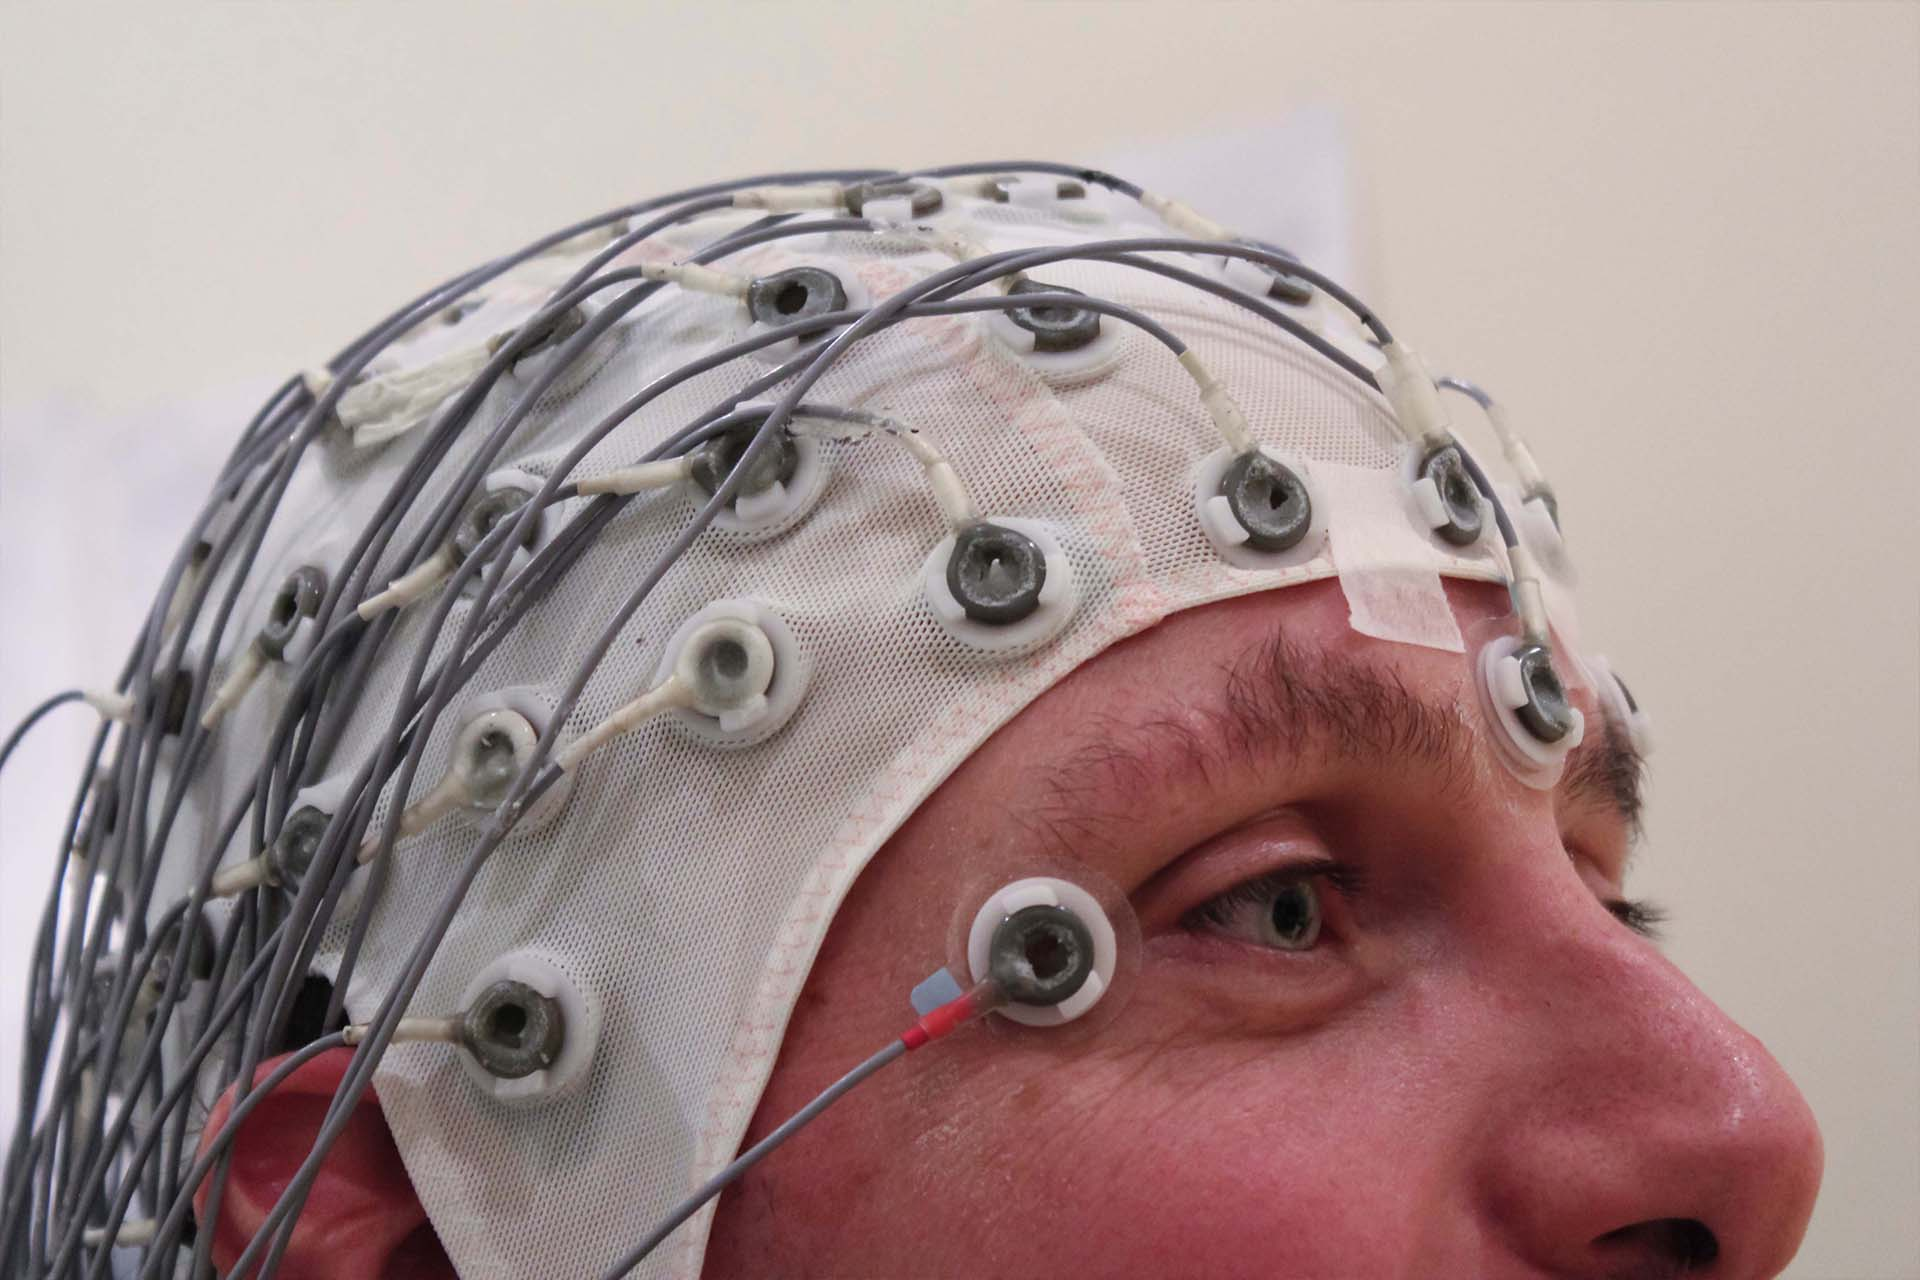
\includegraphics[width=\textwidth]{../images/introduction/wet_eeg.jpg}
        \captionsetup{width=0.9\linewidth}
        \captionsetup{justification=centering}
        \caption{Medical-grade \gls{eeg} measuring equipment that uses wet electrodes which are each connected to a separate main board via a long cable. Image from Chris Hope, CC BY 2.0, via Wikimedia Commons.\\ \hfill}
        \label{fig:example_eeg_measuring_devices_medical_bulky}
    \end{subfigure}
    \hfill
    \begin{subfigure}{.48\textwidth}
        \centering
        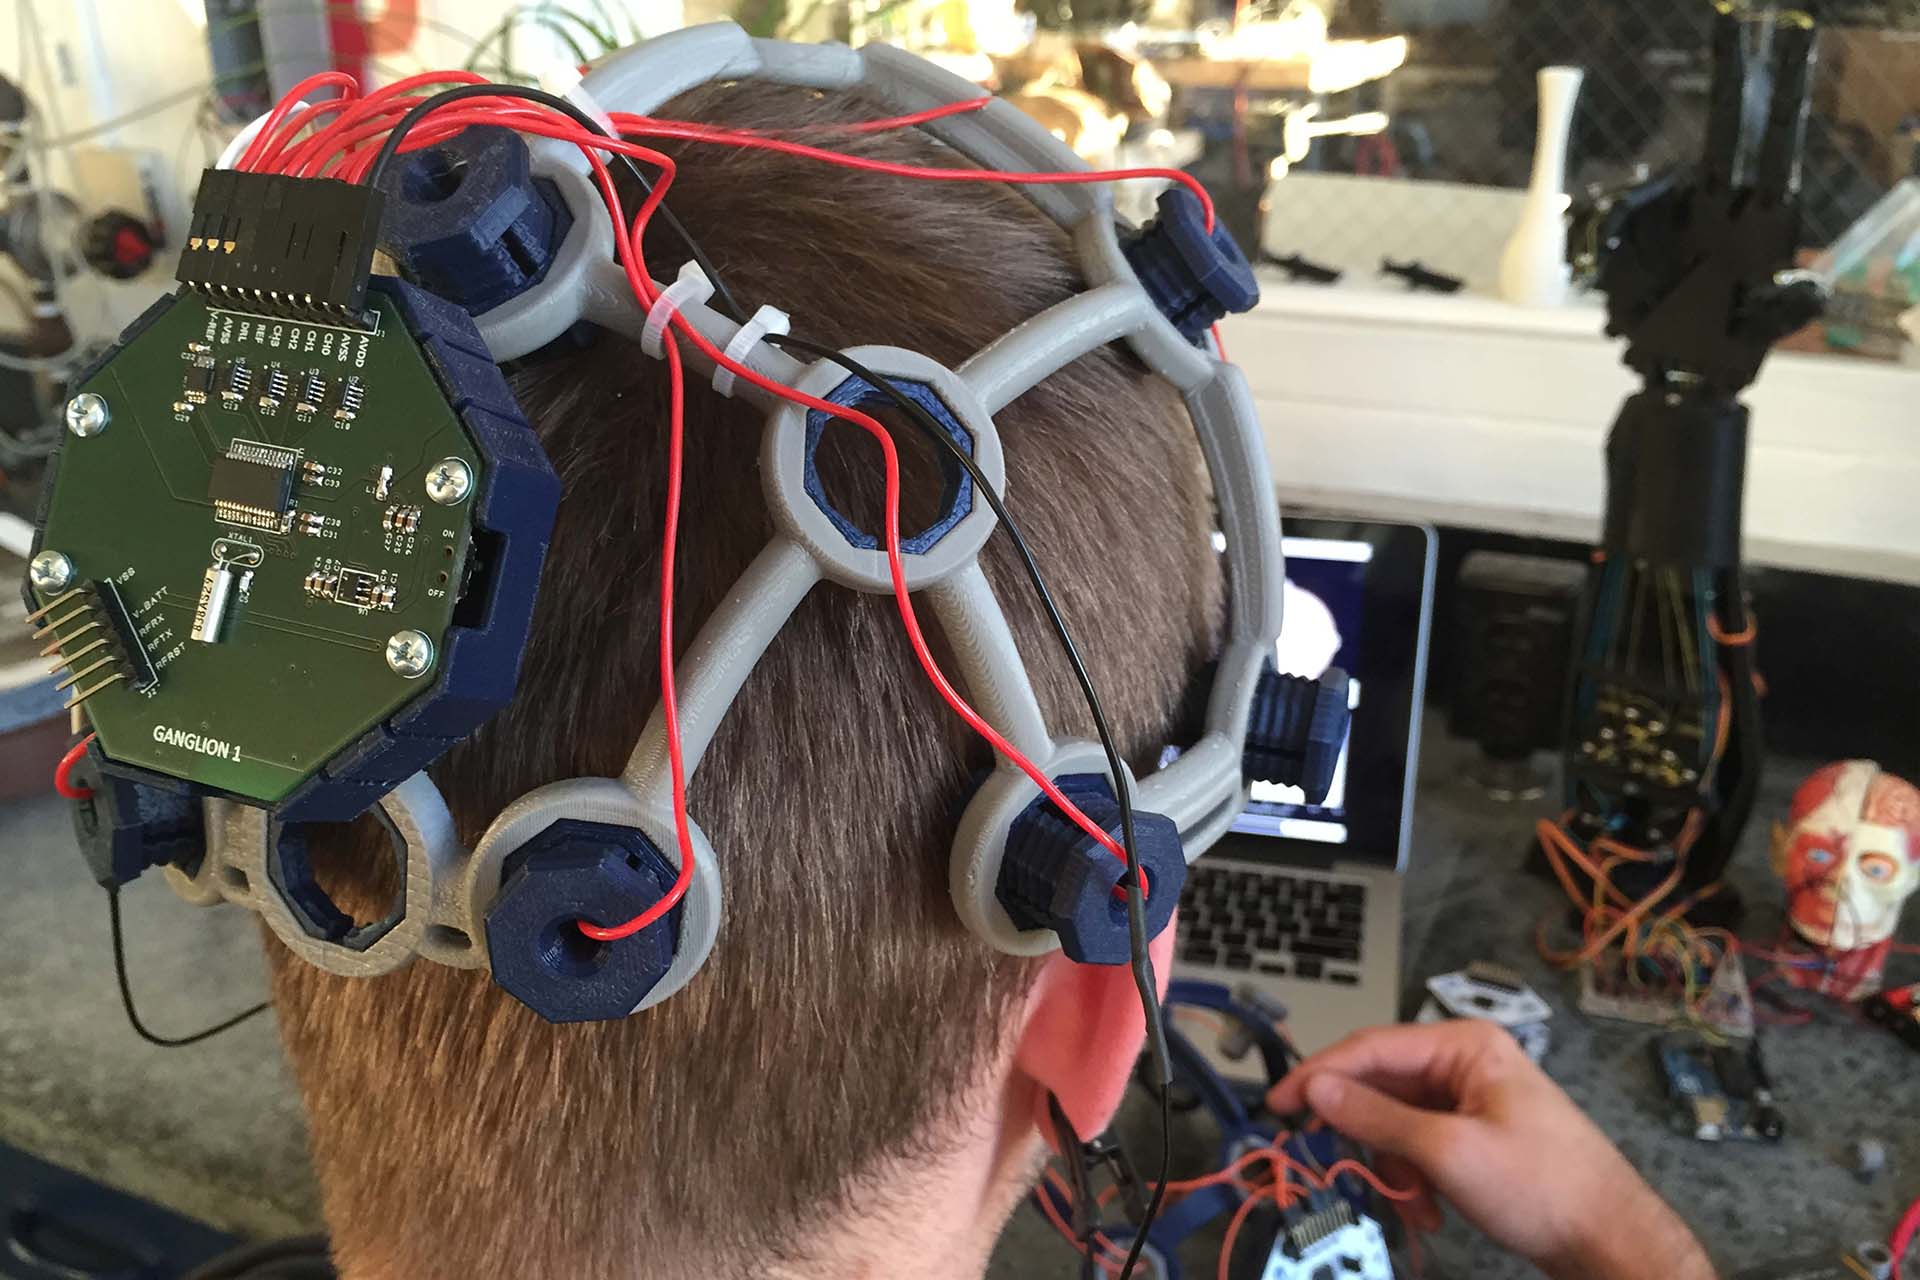
\includegraphics[width=\textwidth]{../images/introduction/openbci.jpg}
        \captionsetup{width=0.9\linewidth}
        \captionsetup{justification=centering}
        \caption{Commercial-grade \gls{eeg} measuring device that uses dry electrodes with active amplification connected to an attached wireless controller board. Image from Conorrussomanno, CC BY-SA 4.0, via Wikimedia Commons.}
        \label{fig:example_eeg_measuring_devices_commercial_clean}
    \end{subfigure}
    \captionsetup{width=0.9\linewidth}
    \captionsetup{justification=centering}
    \caption{The contrast between medical-grade \gls{eeg} measuring equipment and a consumer-grade alternative.}
    \label{fig:example_eeg_measuring_devices}
  \end{minipage}  
\end{figure}

% | | | | | | | | | | | | |

\subsubsection{Algorithmic improvements for non-invasive EEG measuring equipment}
\label{subsubsec:bci_gaining_popularity_better_measuring_software}

Whilst hardware improvements has made the collection \gls{eeg} data more affordable, reliable and accurate, one important issue still remains.
Even with the best active wet electrodes, The contrast between spatial and temporal resolution is enormous.
\Gls{eeg} is known to have a good temporal resolution but rather poor spatial resolution.
A good spatial resolution would mean that the measurement from electrodes corresponds only to a small, known region of the brain, typically underneath that electrode.
Such a correlation is helpful as it reduces noise and increases interpretability of the signal.
It also allows for fewer electrodes to be used if only the activity of certain areas of the brain is of interest.

\begin{figure}[ht]
    \centering
    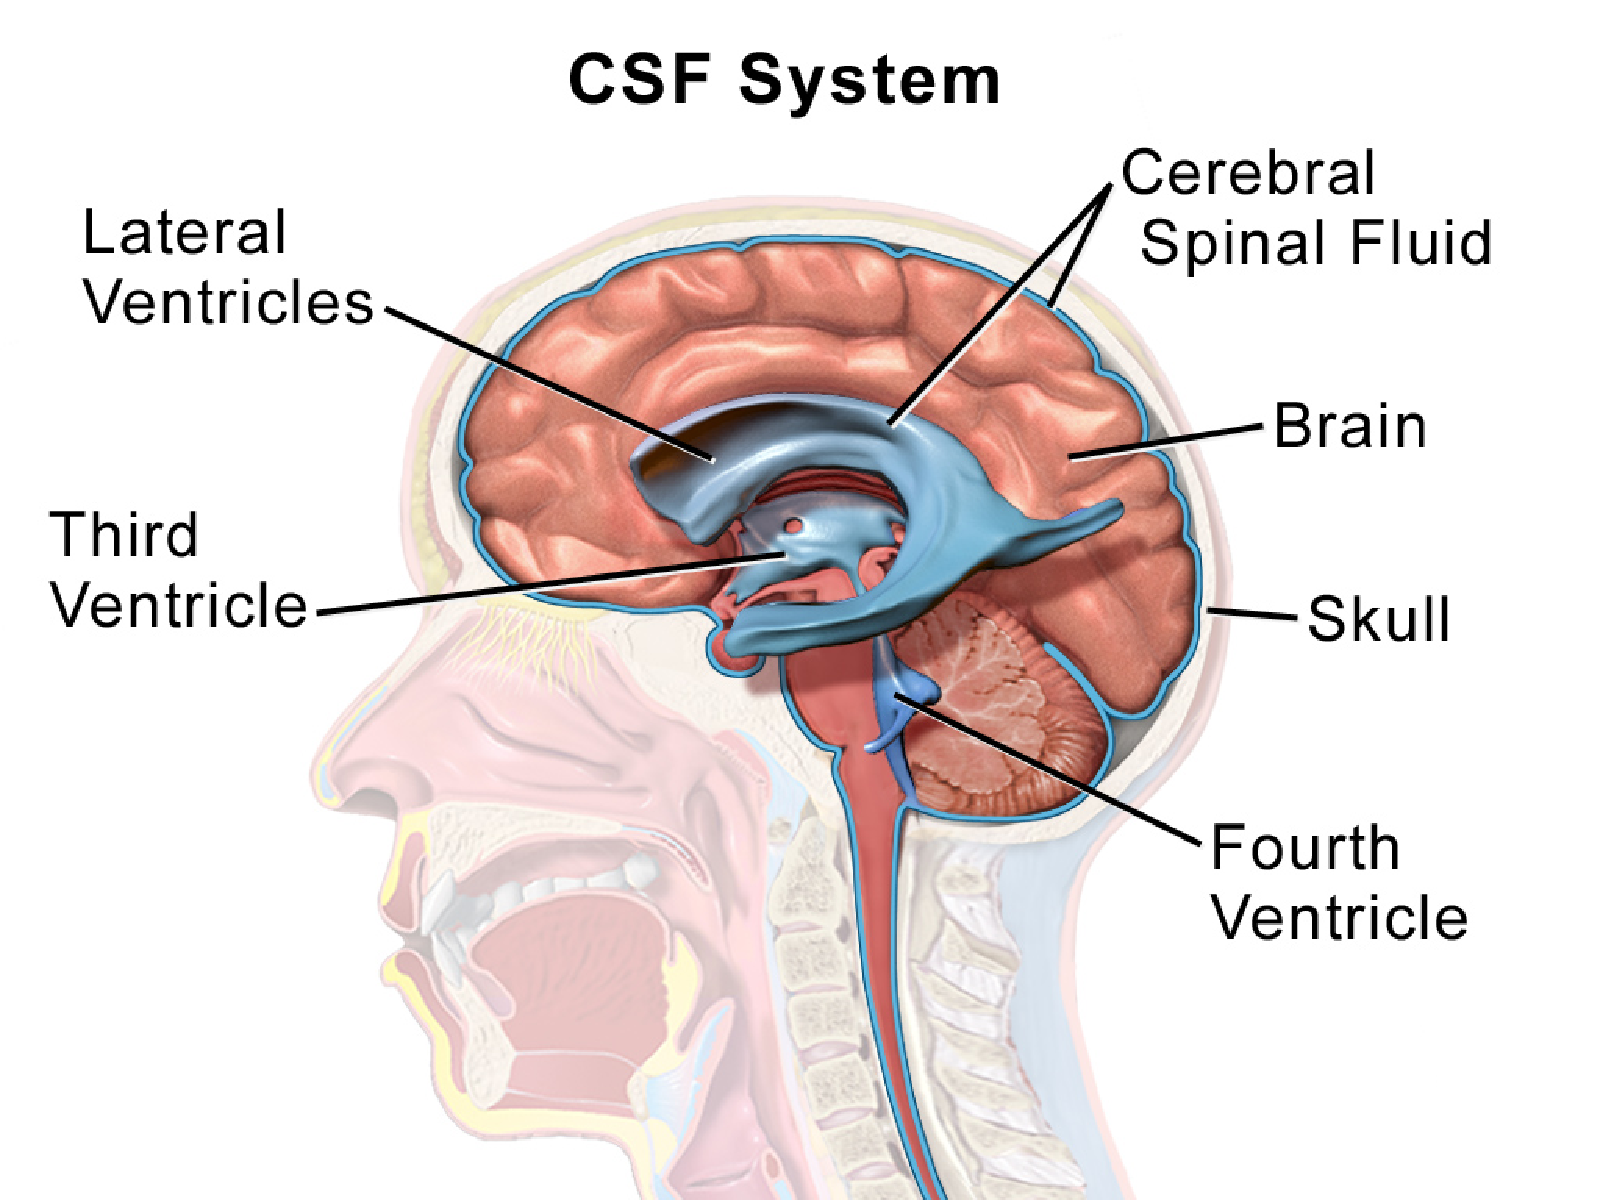
\includegraphics[width=0.7\linewidth]{../images/introduction/brain_anatomy.pdf}
    \captionsetup{width=0.7\linewidth}
    \captionsetup{justification=centering}
    \caption{The anatomy of the human head, specifically of the cerebrospinal system. Non-invasive \gls{eeg} measuring equipment is placed on the scalp, causing signals from the brain to be blocked by the skull and \glsfirst{csf} among other structures. Free to use Figure by Blausen.com staff \citep{figure_blausen}.}
    \label{fig:brain_anatomy}
\end{figure}

Thus, many attempts have been made at improving spatial resolution of \gls{eeg} but it has been proven to be a challenging task \citep{spatial_resolution}.
Besides potential noise of the measurements, this is also caused by the anatomy of the human head.
Remember that the electrodes used for non-invasive \gls{eeg} measuring are placed on the scalp, the skin of the human head.
As shown in Figure \ref{fig:brain_anatomy}, besides the scalp, different structures such as the skull and \glsfirst{csf} are in between the electrodes and the actual brain.
These components \textit{blur} and \textit{disperse} the perceived brain-signal, making it hard to track where the measured signal came from when looking at the electrical activity on the scalp.

Whilst increasing the number of electrodes placed on the skull physically limits the region under one single electrode, it doesn't guarantee an improve in spatial resolution.
Indeed, clever processing algorithms are required to correct for overlapping signals between electrodes so that the overlapped signal is correct for and the effective spatial resolution is improved.
Besides this, there is also the issue that decreasing the distance between electrodes introduces the need for placing more electrodes to cover the entire region of the brain.
This increases cost, lowers user comfort and decreases the visual acceptance of the system.
Another issue with increasing the number of electrodes and decreasing the spatial resolution means that the alignment of the electrodes on the skull is now even more prone to errors and change over time, e.g. due to movement of the user.
This makes the need for a professional higher, which is also detrimental with respect to Wolpaw's criteria for a perfect \gls{bci}.

\Citet{spatial_resolution} has found 19-electrode EEG systems to have a highly varying spatial resolution in the 20 to 40 $cm^3$ range.
Systems with 129 electrodes were found to have a spatial resolution of around 6 to 8 $cm^3$ \citep{spatial_resolution} when also using algorithmic tricks to further improve spatial resolution.
However, according to \citet{neurons_book}, around $10^7$ parallel pyramidal neurons reside in each $cm^3$ of the brain cortex.
This means the acquired data is still obtained from a incredibly large number of neurons even in the best spatial resolutions.

Whilst hardware improvements in both electrodes and headsets for better placement might improve the spatial resolution further, the spatial resolution improvements possible through hardware have been plateauing.
As was the case for the comparison between few and many electrode systems by \citet{spatial_resolution}, appropriate algorithms have to be used to effectively increase the spatial resolution.
Recently, these techniques often rely on using Laplacians \citep{improve_eeg_spatial_laplacian1, improve_eeg_spatial_laplacian2, improve_eeg_spatial_laplacian3}, although other approaches using for example \glspl{cnn} have been proposed \citep{improve_eeg_spatial_cnn}.
These techniques also have the added benefit of cleaning the time-varying signal as described by \citet{improve_eeg_spatial_comparison}.

% | | | | | | | | | | | | |

\subsubsection{Invasive BCIs try to combat the issues of EEG}
\label{subsubsec:bci_gaining_popularity_better_measuring_invasive}

The previous parts discussed how non-invasive \gls{eeg} measurements have been improved.
However, alternatives to \gls{eeg} exist for measuring brain signals, some of which are further discussed in Section \ref{subsec:biomedical_signals_measuring_modalities}.
Most notable in recent years is measuring modalities that rely on capturing brain signals by equipment directly inserted into the human body, making it an invasive approach.
One such example of an invasive measuring modality is \gls{ecog} and the most popular invasive \gls{bci} at the moment is the one proposed by \citet{neuralink_whitepaper}.
The white paper by \citet{neuralink_whitepaper} has shown that invasive \glspl{bci} could greatly exceed the data quality and visual aesthetics of even the best non-invasive alternatives.
As further discussed in \ref{subsec:biomedical_signals_measuring_why_eeg}, this invasive method places flexible electrodes directly inside the skull.
These electrodes are invisible to the human eye with the only visual component being a rechargeable wireless transmitter that is magnetically attached to the skull.
Neuralink's final aim is to make the brain-signal measuring equipment completely invisible to the human eye.

\citet{neuralink_whitepaper} has built robots to insert the electrodes inside the skull in a very precise location without the need for an open-skull operation or even anaesthesia.
This allows for a magnitude more electrodes to be installed and is expected to suffer far less from noise resulting in a far greater temporal and spatial resolution compared to \gls{eeg}.
This suggests that invasive systems are superior to non-invasive alternatives, but the fact that they are more permanent, far more expensive and invasive gives rise to technical and ethical questions.
These ethical questions are further discussed in Section \ref{sec:bci_ethical}.
From a technical standpoint, maintaining and upgrading a non-invasive \glspl{bci} is far simpler and cheaper.
The fact that you are inserting foreign objects into the brain also introduces far more health risks than non-invasive systems do.
Convincing the user to put on a headset that can be removed will also be far easier than convincing the user to get a \gls{bci} permanently implemented in their skull.

It has also been shown that the theoretical more precise temporal and spatial resolution doesn't linearly correlate with improved \gls{bci} accuracy/control, rather it seems to plateau relatively quickly with current state-of-the-art signal processing and classification techniques \citep{dropping_curve_eeg_lectrodes, more_electrodes_not_better}.
Some critics point to the dropping curve found by \citet{dropping_curve_eeg_lectrodes} to conclude that the increased electrode amount and reachable neurons achieved by \citet{neuralink_whitepaper} don't have a direct impact on the usability of \glspl{bci} in real-world applications.
Because of these aspects, the ease-of-use appeal and far cheaper price for non-invasive alternatives still outweigh the benefits offered by invasive methods for almost all but highly medical applications, at least in the opinion of the writer of this thesis.
Nevertheless, future improvements in signal processing and classification techniques could prove invasive methods to be far superior for \gls{bci} applications and the mechanical achievements so far are not to be underestimated.
An invasive system is also promising concerning Wolpaw's definition of a perfect \gls{bci} discussed in Section \ref{sec:bci_introduction}.
Once installed, it would ideally require no more assistance from a professional, is aesthetically acceptable as it can be invisible to the human eye, has signs of being far more reliable than \gls{eeg} and more.

% | | | | | | | | | | | | |

\subsubsection{Summarizing the improvement of measuring facilities}
\label{subsubsec:bci_gaining_popularity_better_measuring_summary}

Since \glspl{bci} rely solely on brain signals to operate, the measuring facilities for acquiring data of those brain signals have a direct impact on the capability of those systems.
As was discussed in this section, the most commonly used modality for non-invasive data acquisition, \gls{eeg}, has benefited from both hardware and software improvements.
From a hardware point of view, the switch to dry electrodes using active amplification and wireless connection to a computational unit has made \glspl{bci} more favourable concerning Wolpaw's criteria for a perfect \gls{bci} \citep{bluetooth_evaluation, wet_vs_dry, active_electrode_explained}.
From a software perspective, clever algorithms have enabled preprocessing of the signal to improve spatial resolution \citep{improve_eeg_spatial_laplacian1, improve_eeg_spatial_laplacian2, improve_eeg_spatial_laplacian3, improve_eeg_spatial_cnn}.
Improving the spatial resolution can also positively affect the temporal resolution due to inherent noise reduction as discussed by \citet{improve_eeg_spatial_comparison}. 
As is further discussed in Section \ref{subsec:processing_signals_general_pipeline_preprocessing}, other prepossessing techniques have also been introduced and refined further aiding in improving the data quality. 

% - - - - - - - - - -
% better hardware
% - - - - - - - - - -

\subsection{More powerful, affordable and portable equipment}
\label{subsec:bci_gaining_popularity_better_processing}

The improvements in brain signal measuring equipment have likely been influential in the gaining popularity of \glspl{bci} as it provides more precise data more affordably.
However, having the possibility of obtaining clean data is only part of the way to a perfect \gls{bci} system.
Other improvements concerning computational power, affordability and portability have also played an important role in \gls{bci} research, contributing to the rise of popularity in the process.

% | | | | | | | | | | | | |

\subsubsection{The emergence of faster and cheaper hardware}
\label{subsubsec:bci_gaining_popularity_better_processing_cheaper}

As chapter \ref{ch:processing_signals} will discuss in greater detail, working with \gls{eeg} data, or other forms of brain signal data can require computationally very heavy operations to achieve desired processing results of that data.
Luckily, together with the improvements in state-of-the-art measuring equipment, there is also an emerging supply of less accurate but far more affordable and portable \gls{eeg} measuring equipment.
Due to Moore's law \citep{moores_law} and other advancements, \glspl{cpu} and other computational hardware have also seen massive improvements in computational power.
This has made algorithms previously requiring expensive specialized computational hardware possible on the average personal computer.
All of these factors have made \gls{bci} applications, which were previously limited to lab environments with a high financial cost, accessible to a far broader public.
The availability of open-source datasets for common tasks related to brain signals has also allowed computer scientists to experiment in the field without additional hardware cost \citep{eeg_data}.

% | | | | | | | | | | | | |

\subsubsection{Splitting BCIs into multiple major components for portability and reusability}
\label{subsubsec:bci_gaining_popularity_better_processing_split_into_components}

Early attempts at making \glspl{bci} more portable and affordable include those by \citet{early_bci_drowsiness} and \citet{early_bci_multimedia}.
In essence, these applications rely on separating the data acquisition process and data processing into two standalone systems connected over Bluetooth.
Remember from Section \ref{subsec:bci_gaining_popularity_better_measuring} that Bluetooth is an open standard for wireless communication that has seen improvement in the last couple of years.
Dividing a \gls{bci} system in a data acquisition and data processing system allows for creating a lightweight measuring device to be placed on the user's head, with a heavier and bulkier computational unit to process the signals which ideally is still pocket-able.
The latter was not a trivial task and introduced the need for custom hardware at the time.
\citet{early_bci_drowsiness} used a custom-made \gls{dsp} for the task whilst \citet{early_bci_multimedia} opted for a more general \gls{fpga} based \gls{dsp}.
Whilst these were great demonstrations of how the technology could be used outside the lab, the actual usage for a bci detecting driver's drowsiness \citep[as proposed in the paper by][]{early_bci_drowsiness} and allowing multimedia control \citep[as proposed in the paper by][]{early_bci_multimedia} was rather limited.
The idea of custom-made and possibly proprietary processing hardware which focuses on a single task is also very limiting, although it does have commercial benefits.

What did stick, was the idea of splitting the hardware into two standalone parts, a wireless \gls{eeg} measuring device and a processing unit.
As discussed in Section \ref{subsec:bci_gaining_popularity_better_measuring}, a wireless connection between these two components is also favoured when taking into account Wolpaw's criteria on a perfect \gls{bci}.
It also makes it possible for smaller research teams or even individuals with a certain specialisation to take part in the highly interdisciplinary field by not requiring knowledge of all components but just the one that is of interest.
As an example, it enables computer scientists to purchase off-the-shelve affordable \gls{eeg} measuring hardware and communicate with it through provided libraries for their favourite programming language.
In most cases, the personal computer they already own is powerful enough for the experiments, especially for offline systems.
This allows for reusing existing hardware which is great from a financial perspective.
Section \ref{subsec:biomedical_signals_measuring_equipment} discusses some of the \gls{eeg} measuring equipment available on the market.
It is noted that \gls{eeg} measuring hardware is not strictly needed for a computer scientist as researchers such as \citet{eeg_data} have made excellent free-to-use \gls{eeg} datasets available.

With the introduction of the iPhone in 2007, it didn't take long for researchers to explore the idea of using a mobile phone as a processing unit for a \glspl{bci}.
\citet{early_bci_phone} were one of the first to explore this idea, with a \gls{ssvep}-based \gls{bci}.
Section \ref{subsec:biomedical_signals_brain_signals_measurable_brain_activity} will go into further detail on the types of measurable brain-signals.
In essence, such a system relies on a category of brain signals that are often easy to detect but require a specific stimulation.
This type of system can be used for a wide variety of applications.
Imagine an audio-guided tour in a museum where visitors only need to stare at a screen next to an item of interest to start hearing the explanation of that item.
This could be achieved with only a couple of dry electrodes placed on the skull in a headset that also provides the audio to the visitor.
This headset could then be connected over Bluetooth to the visitor's phone running an app for the museum tour.
The technology needed for such a system would lean close to that of so-called \textit{P300 spellers}, which have already been heavily studied \citep{p300_spellers_review, p300_keyboard_flashing, p300_spellers}.
Such a system would also fit perfectly with Wolpaw's definition of a perfect \gls{bci}, albeit oriented to a commercial setting rather than a medical one.

% | | | | | | | | | | | | |

\subsubsection{Making BCIs a one-in-all device again for profitability}
\label{subsubsec:bci_gaining_popularity_better_processing_profitibility}

Whilst the advantages of using the computational power of devices a customer already owns are clear, it also imposes some disadvantages.
For one, the varying type of computational devices is bound to give varying performance results, compatibility issues and overall limits the guarantee of a pleasing \gls{ux}.
Adding to this, the measuring equipment and processing equipment can't be connected from the factory resulting in an experience that is not plug-and-play.
From a commercial perspective, it would be easier if the system was all-inclusive and possibly patentable. 

Recent trends in computing hardware where manufacturers are shifting away from general all-purpose \glspl{cpu} and them developing their own custom \gls{cpu} architectures have shown that custom chips can outperform their general counterparts.
Patenting the architecture of those chips is possible making it commercially interesting.
Apple's mac M series processors announced in 2020 are one such recent example.
These M series processors have a neural engine that is stated to accelerate the time needed for \gls{ml} tasks\footnote{\url{https://nr.apple.com/dH8i4U3v2w}}.
\Glspl{gpu} used for autonomous driving systems also differ from general-purpose \glspl{gpu}.

Because of this, the author of this paper believes custom-made chips could create a future where the headset has a directly integrated processing unit once again.
Whilst this would make for a more attractive package for the customer and give commercial advantages to the manufacturer, it would be disadvantageous for research purposes.
The manufacturer could limit the possibilities of using the \gls{bci} for different purposes, patent promising hardware and more.
Another possible route the author of this paper sees is the use of cloud computing and fast 5G connections to also create a more simple user experience that doesn't require Bluetooth tethering to a close-by processing unit.
This approach would still leave a separation between measuring hardware and processing hardware making changes to any of the two independently easier.
Concerning Wolpaw's criteria of a perfect \gls{bci}, these approaches would also be acceptable.
This belief of switching back to all-in-one devices or using a cloud service for processing the data is further endorsed by the findings of \citet{bci_review_arnau}.
In their systematic review of \gls{bc} systems, eight of the 46 studied papers used embedded hardware and one used cloud solutions.

% | | | | | | | | | | | | |

\subsubsection{Summarizing the improvements on computational power, affordability and portability}
\label{subsubsec:bci_gaining_popularity_better_processing_summary}

To summarize, due to Moore's law \citep{moores_law} and other advancements, \glspl{cpu} among other computational hardware have seen massive improvements in computational power.
This increase in computational power has enabled more advanced processing of the data on more affordable and portable hardware.
Early attempts at making \glspl{bci} more portable and affordable focused on splitting the brain signal measuring equipment from the data processing equipment \citep{early_bci_drowsiness, early_bci_multimedia}.
The system by \citet{early_bci_phone} was one of the earliest examples of a true portable \gls{bci}-system that was affordable and relied on a smartphone as a processing unit.
It showed how working with \glspl{bci} can be done using cheap and general-purpose hardware.
The research was published at a turning point for \glspl{bci} where publication numbers on \gls{bci}-related papers started rising.
This hints that the increased affordability and portability combined with more computational power played an important factor in the rise of interest in \gls{bci}. 
The rise of \gls{bci}-related papers is illustrated in Figure \ref{fig:bci_publications} based on data by \citet{bci_progress_overview}.
\Citet{bci_review_arnau} found that papers on \gls{bc} systems using \gls{dl} have seen a steady increase over the last five years as well. 

In the future, as \glspl{bci} see more commercial applications, this separation of a \gls{bci} in a measuring component and processing component might reverse to an all-inclusive device.
This has potential downsides for scientific research but makes commercial sense.
The replacement of physical computational units in close proximity to cloud solutions is another possible evolution.

\begin{figure}[ht]
    \centering
    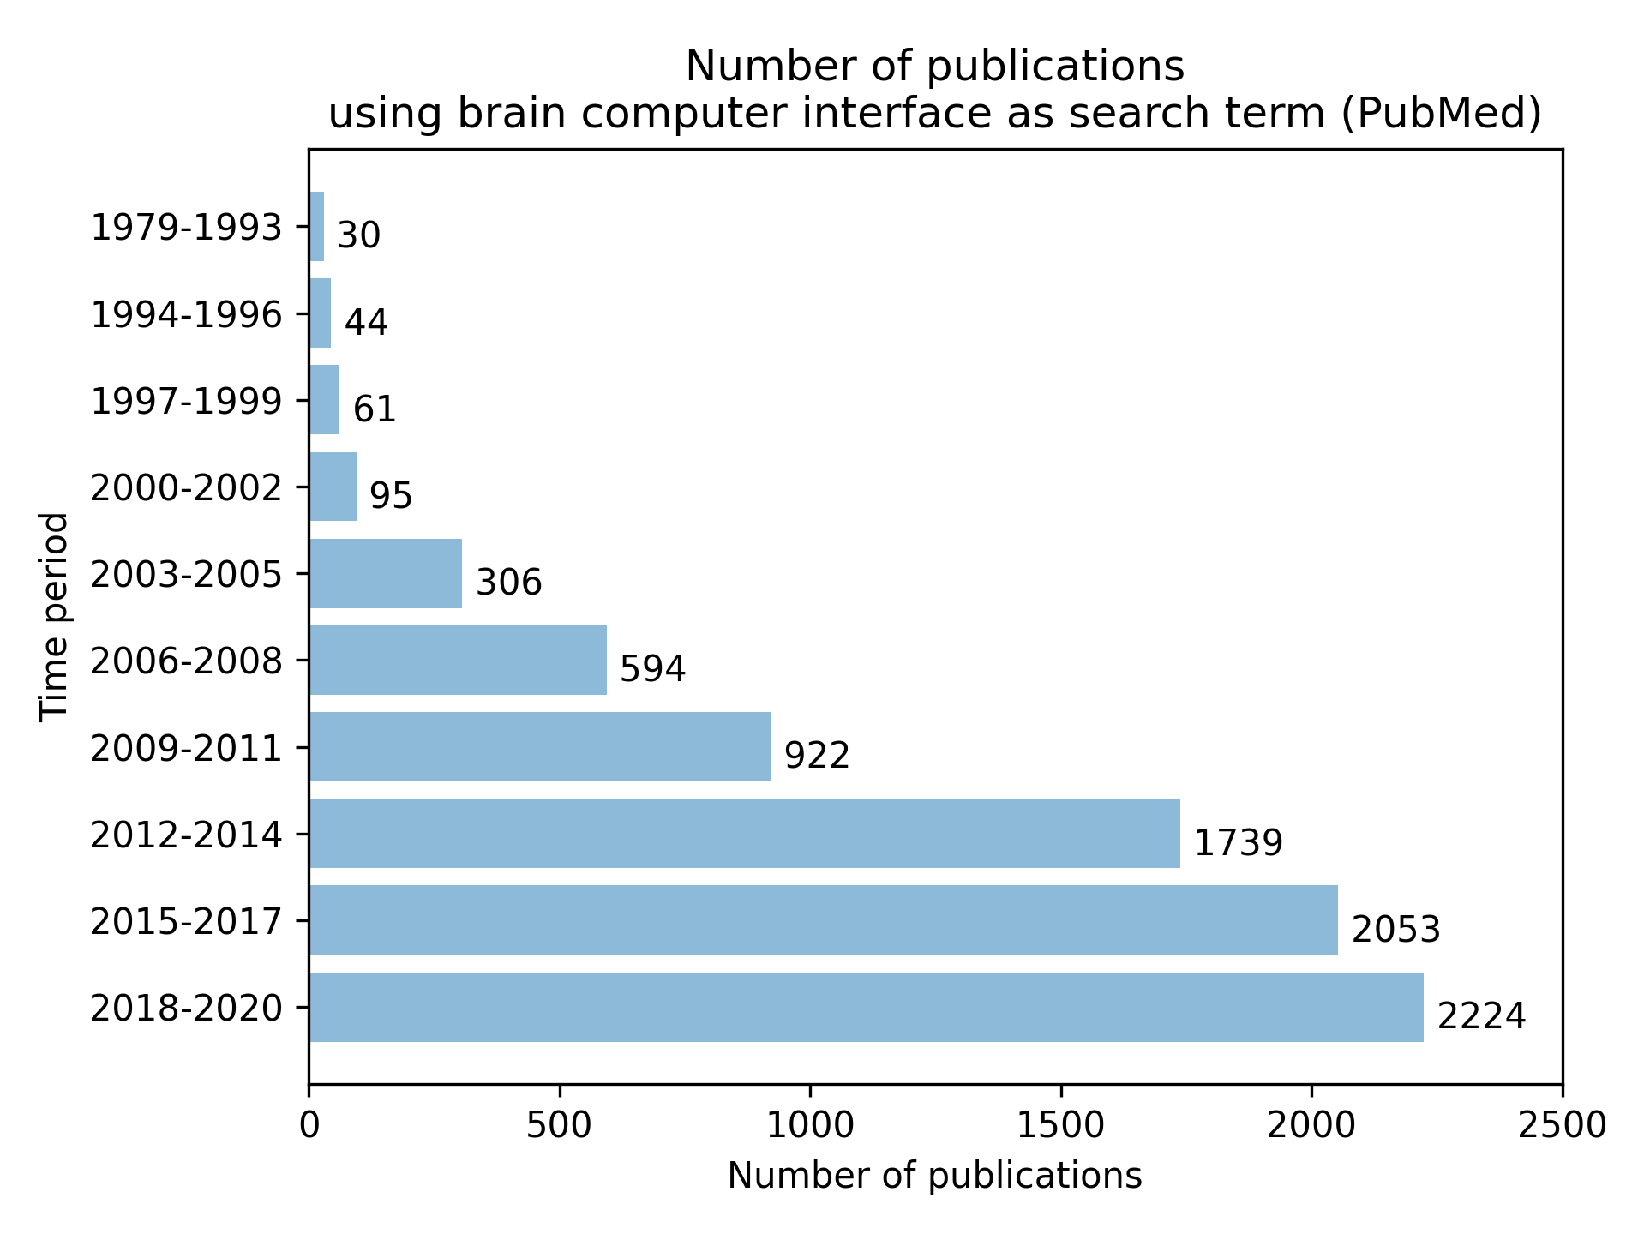
\includegraphics[width=0.8\linewidth]{../images/introduction/papers_on_bci.pdf}
    \captionsetup{width=0.7\linewidth}
    \captionsetup{justification=centering}
    \caption{Number of \gls{bci}-related papers over time. Based on data by \citet{bci_progress_overview} obtained by searching PubMed using the keyword: "brain-computer interface".}
    \label{fig:bci_publications}
\end{figure}


% - - - - - - - - - -
% better software
% - - - - - - - - - -

\subsection{Specialized data processing techniques}
\label{subsec:bci_gaining_popularity_improved_data_processing}

\glsreset{dl}

The previous sections \ref{subsec:bci_gaining_popularity_better_measuring} and \ref{subsec:bci_gaining_popularity_better_processing} discussed how both measuring and computational hardware have seen recent improvements.
Another important part of the puzzle is the algorithms that convert data from the now more user friendly measuring devices to useful actions using the now more powerful, affordable and more portable computational hardware.
Most of these algorithms are data-driven classifiers that use \gls{ml} techniques.
In more recent years, \gls{dl} techniques and alternative approaches have been incorporated in the \gls{bci} pipeline as well, which has been proven to be very successful. 
Chapter \ref{ch:processing_signals} discusses commonly used techniques in more detail and multiple \gls{ml} and \gls{dl} based \gls{bci} pipelines are discussed in later chapters of this thesis.
This section gives a more high-level summary of recent developments in the \gls{ai} field that have likely contributed to the rise in popularity of \glspl{bci}.

% | | | | | | | | | | | | |

\subsubsection{Postponing another AI winter}
\label{subsubsec:bci_gaining_popularity_improved_data_processing_no_ai_winter}

\Glsfirst{ml} and \glsfirst{dl} are techniques that fall under the \gls{ai} umbrella.
These techniques are being used as buzzwords in a whole suite of applications and it seems as if every week there is yet another big promise or threat related to \gls{ai} discussed in major news outlets.
Recent examples that have shown the world what new techniques in this field are capable of include the Go champion beating computer algorithm by \citet{alphago}, the impressive text generation model GPT-3 by \citet{GPT3} and the image generation model DALL-E by \citet{dall_e}.
This abundance of new achievements and an overall high public interest in anything that mentions buzzwords from the \gls{ai} umbrella has caused a long lasting \gls{ai} summer since the last \gls{ai} winter of the late 1980s and early 1990s.
Such an \gls{ai} summer means that there is incredible amount of funding available for improving \gls{ml} and \gls{dl} techniques among others.
This in term causes further advancements in the field of \gls{ml} and \gls{dl} which results in more impressive achievements.

However, an \gls{ai} summer also implies that an \gls{ai} winter will inherently return.
An \gls{ai} winter is a period of time where the interest in the field is reduced and thus funding and research is limited.
As discussed by \citet{new_ai_winter}, such an \gls{ai} winter may be relatively close.
This is in part due to new regulations and public backlash on the more questionable but highly profitable applications \gls{dl} is involved in.
A recent example of this is the controversy surround Clearview AI.
Here, state-of-the-art \gls{dl} image recognition algorithms are used on billions of images collected from all over the internet, including social-media platforms, to recognize almost anyone with a public profile linked to them.
As further discussed by \citet{clearview_ai}, this technology conflicts with many EU laws yet was used by multiple police departments.
Adding to this, new regulatory changes are being proposed to limit the use of algorithms which lack explainability and interpretability \citep{eu_ai_blackbox_report, explainable_ai_policy}.
This challenges many \gls{ml} and \gls{dl} approaches currently used as explained further in Section \ref{subsec:processing_signals_common_issues_exaplainable}.

Nevertheless, there is still a high amount of resources being put into \gls{ml} and \gls{dl} research.
Throughout history, these technologies have been linked with the biomedical setting a lot.
As explained by \citet{dl_and_biomedical}, \gls{dl} and biomedical data have directly influenced each other's evolution's since the 1980s.
Because of this, applications that process biomedical data have been an important factor at prolonging the current \gls{ai} summer.
Since \glspl{bci} use biomedical data as well, they have been one of the applications keeping interest in \gls{ml} and \gls{dl} research high.
This is in part due to the science-fiction properties \gls{bci} systems have creating a lot of public interest as already discussed when talking about Elon Musk's Neuralink in Section \ref{subsec:bci_gaining_popularity_big_tech}.
Thus, \gls{bci} systems, which rely heavily on \gls{ml} and \gls{dl}, are one of the research areas in these technologies that are so promising they help prolonging the current summer of \gls{ai}.

% | | | | | | | | | | | | |

\subsubsection{Improved and new ML and DL concepts have enabled more capable BCI systems}
\label{subsubsec:bci_gaining_popularity_improved_data_processing_better_ml_dl}

Most of the main concepts from both \glsfirst{ml} and \glsfirst{dl} are already multiple decades old.
As \gls{dl} is a subset of the \gls{ml} techniques, pipelines for using these techniques are very similar.
To illustrate this, a general pipeline of a \gls{cad} system used for classification is given in Figure \ref{fig:cad_pipeline} and commonly used techniques are discussed below.
It is noted that besides classification tasks, some regression problems for \gls{cad} systems exist as well.
However, such regression problems are far less common in \gls{bci} systems relying on \gls{eeg} with the systematic review article of \citet{bci_review_arnau} only finding articles on classification problems for such systems.
Because of this, this thesis focuses on classification problems.
\gls{cad} systems are used extensively in hospitals for the interpretation of biomedical images and have been studied ever since computers were invented.
The most common example of a \gls{cad} system is the classification of lung images as being either from a lung cancer patient or not, often also highlighting the nodules used for this classification.
These pipelines are very similar to the ones used for \glspl{bci}, which is further discussed in Section \ref{sec:processing_signals_general_pipeline}.

\begin{sidewaysfigure}
    \centering
    \begin{subfigure}{\textwidth}
        \centering
        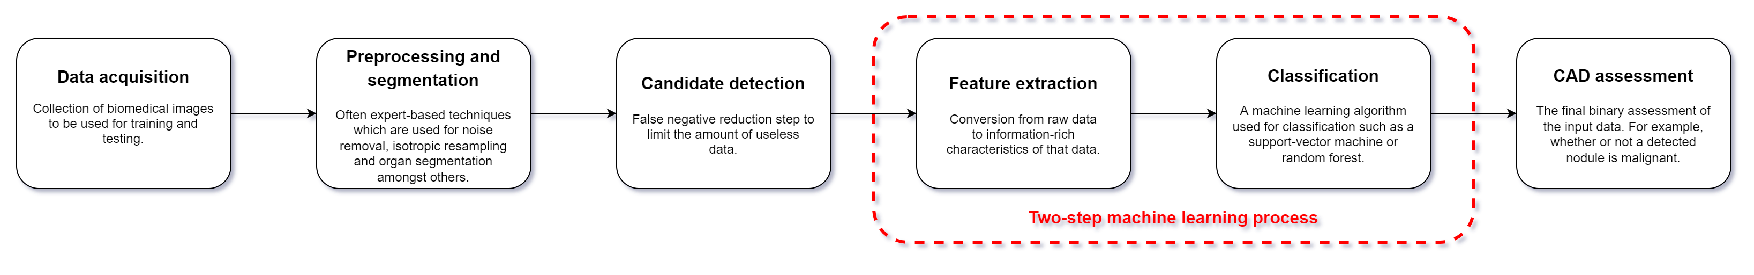
\includegraphics[width=\textwidth]{../images/introduction/cad_pipeline_ml.pdf}
        \captionsetup{width=0.9\linewidth}
        \captionsetup{justification=centering}
        \caption{General pipeline for \gls{ml} based \gls{cad} system.}
        \label{fig:cad_pipeline_ml}
    \end{subfigure}
    \hfill
    \begin{subfigure}{\textwidth}
        \centering
        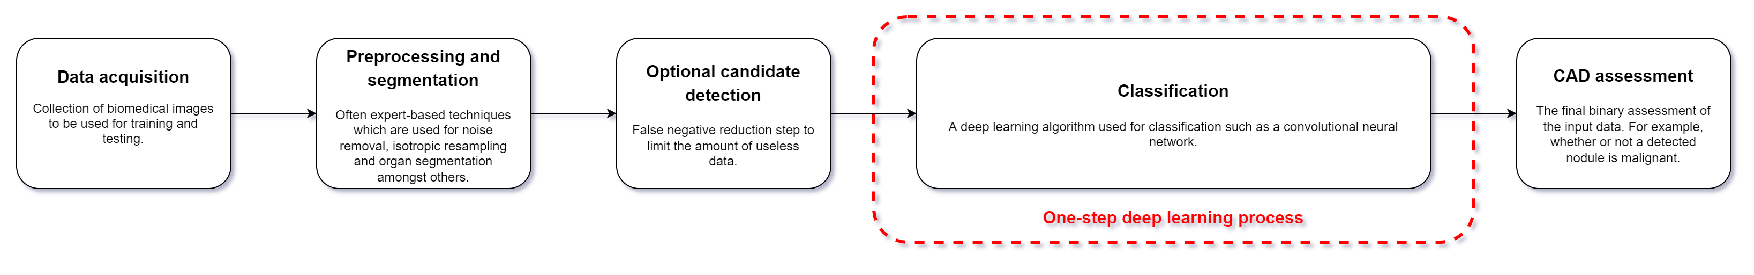
\includegraphics[width=\textwidth]{../images/introduction/cad_pipeline_dl.pdf}
        \captionsetup{width=0.9\linewidth}
        \captionsetup{justification=centering}
        \caption{General pipeline for \gls{dl} based \gls{cad} system.}
        \label{fig:cad_pipeline_dl}
    \end{subfigure}
    \captionsetup{width=0.9\linewidth}
    \captionsetup{justification=centering}
    \caption{General pipelines of a \gls{cad} system used for classification. A \gls{ml} approach is called a two-step approach as it exists from feature extraction and classification. A \gls{dl} approach is called a one-step approach as it combines both of these steps into a singular classification algorithm.}
    \label{fig:cad_pipeline}
\end{sidewaysfigure}

Traditional \gls{ml} is a commonly used name for the collection of \gls{ml} techniques that are not \gls{dl}.
Such traditional \gls{ml} rely on a \textit{two-step} process where there is both a feature extraction step and a regular classification step as is visualised in Figure \ref{fig:cad_pipeline_ml}.
Feature extraction is the process of representing the often highly dimensional and unstructured raw data using characteristic properties.
These representations are often derived from expert knowledge and are chosen by the designer of the system rather than learned from data.
With respect to a \gls{cad} system for classifying if a patient has lung cancer, these features might be the size of nodules in the lung, a metric of how round these nodules are, the \gls{hu} of certain parts of the lungs and more.
These features are then used for learning by a traditional \gls{ml} classifier.
The true challenge in these two-step traditional \gls{ml} systems lies in finding appropriate features, which can be a very time-consuming task that requires a lot of domain knowledge.
It isn't uncommon for features in \gls{cad} systems to be refined in the span of multiple years \citep{CAD_ml_dl_kbs}.
Section \ref{subsec:processing_signals_general_pipeline_features} discusses the feature engineering step in more detail and Section \ref{subsec:processing_signals_ml_and_dl_ml_classifiers} discusses traditional \gls{ml} in more detail.

Alternatively, a \textit{one-step} approach in \gls{cad} systems denotes the use of \gls{dl} in the pipeline, such as shown in Figure \ref{fig:cad_pipeline_dl}.
\gls{dl} generally differentiates itself from the previously discussed two-step traditional \gls{ml} approach by working directly on the preprocessed data rather than a feature representation of the data.
However, this isn't necessarily the case as feature extraction can still be beneficial for some \gls{dl} methods whilst others might even work better on the raw, non-preprocessed, data.
Section \ref{subsec:processing_signals_ml_and_dl_difference} discusses the difference between traditional \gls{ml} and \gls{dl} in more detail.
Intuitively, \gls{dl} models exist of multiple layers which can be seen as a graph-like structure which becomes deeper as the number of layers increases, hence the name \glsfirst{dl}.
Typically, multiple types of layers are present in a \gls{dl} approach, with the earlier layers focusing on what could be seen as gradual feature extraction steps whilst the later layers are often more tailored towards the classification of those data-driven feature outputs from the previous layers.
Section \ref{subsec:processing_signals_ml_and_dl_dl_classifiers} discusses \gls{dl} and the common variations in more detail.
A \gls{dl} approach is interesting as it can allow for skipping the feature extraction process where good features have to be found by the developer of the system.
Finding such good features can not only be time-consuming but limited expert knowledge can also make creating features that carry enough differentiating information impossible, meaning that even the best classifiers can't learn from them.
Adding to this, \gls{dl} approaches in \gls{cad} systems have also been proven to outperform state-of-the-art \gls{ml} approaches \citep{CAD_ml_dl_kbs}.
However, \gls{dl} models are more challanging in terms of explainability and interpretability as further discussed in Section \ref{subsec:processing_signals_common_issues_exaplainable}.
The challenge in \gls{dl} approaches is finding a suitable model and training it in a way such that it doesn't overfit, a phenomenon further discussed in section \ref{subsec:processing_signals_common_issues_overfitting}.
In a way, \gls{dl} allows a person with limited domain knowledge of the data to obtain a better result as it bypasses the need for manual feature extraction.
However, this is a double-edged sword as limited knowledge of the data increases the risk of bias, overfitting and other potential issues.

Relating this to \glspl{bci}, which have a very similar pipeline, and how the \gls{ml} and \gls{dl} techniques used often originate from older concepts, some of the most common \gls{bci} pipeline components are considered.
A typical traditional \gls{ml} \gls{bci} pipeline often relies on a form of the \gls{csp} technique for feature extraction.
This technique is quite old being introduced by \citet{first_csp} around 30 years ago.
Likewise, the traditional \gls{ml} classification used is often a type of \gls{svm}.
Once again, this technique was first introduced by \citet{first_svm} around 30 years ago.
Over the years, \gls{csp} has evolved and many extensions such as \gls{fbcsp} by \citet{eeg_model_fbcsp} have been introduced.
Likewise, \gls{svm} has seen many extensions and improvements \citep{svm_extension1, svm_history}.
This has resulted in the combination of these two relatively old techniques, but with recent extensions, still performing among the state-of-the-art in \gls{bci} applications using traditional \gls{ml} approaches \citep{bci_competition_review, ml_strats_used_in_papers}.
Likewise, when using a \gls{dl} approach in the \glspl{bci} pipeline, \glspl{cnn} are most commonly used \citep{ml_strats_used_in_papers, bci_review_arnau}.
This technique is again a rather old one, the foundations of which were first described by \citet{first_cnn} over 40 years ago.
Just as the \gls{csp} procedure, \glspl{cnn} have seen multiple extensions and improvements over the year, just as other \gls{dl} approaches.
Most recent and noteworthy developments are works such as that by \citet{eeg_model_hbm} which focuses on proposing \gls{cnn} architectures that can learn from very few samples and for which a described method exists to visualize the model's early layers.
Other improvements, more general to \gls{dl}, have also been made such as the development of new activation functions. \Citet{rl_activation_function_compare} discus how changing the activation function from CReLU to ReLU6 offered a 35\% performance increase while keeping other components fixed for certain experiments relying on a \gls{nn} in a \gls{rl} setting.
Thus, these improved versions of older concepts have enabled far better performance making it possible to create more capable \gls{bci} systems.

This doesn't mean that all approaches used for processing the data in \glspl{bci} rely on decades-old techniques that have improved over the years.
One interesting and relatively new approach is the use of \gls{tl} from drastically different domains.
Previously, \gls{tl} was mostly used in \glspl{bci} to train a model on data which may originate from different users performing similar but not necessarily identical tasks.
This general model is then further refined on a specific patient and task, transferring the knowledge acquired from the previous data to the new data.
When done correctly, this can provide far better performance compared to learning on the new data alone for problems where data is limited \citep{bci_review_arnau}.
As available data specific to \glspl{bci} applications remains limited, some recent research has gone into transferring knowledge from completely different domains to \gls{bci} specific data.
\Citet{tl_cnn_eeg} used a model pretrained on images and transferred it to \gls{eeg} data for a \gls{mi} task with promising results.
Other attempts at transferring knowledge from other domains, such as natural language, have also been made \citep{thesis_wolf}.


% | | | | | | | | | | | | |

\subsubsection{More open-source datasets and BCI related libraries}
\label{subsubsec:bci_gaining_popularity_improved_data_processing_open_source_data_code}

Whilst more affordable and portable measuring hardware has enabled a low-cost solution for researchers to acquire their own data, as discussed in Section \ref{subsec:bci_gaining_popularity_better_processing}, the process of acquiring \gls{bci} related data remains significantly time-consuming and can impose multiple challenges.
As addressed by \citet{bci_review_arnau} many publications don't properly report the data acquisition process, leaving a lot of ambiguity in both the meaning of data labels and how representative of the real-world the data is.
Whilst two papers might discuss a \gls{mi} task as being \textit{imagined left-hand movement}, one might have collected the data in a lab-like environment from a trained user envisioning a single squeezing shut movement of the hand whilst another might have it correspond with any envisioned movement of the fingers on an untrained and non-focused user.
On a legal aspect, as data on brain signals is biomedical data, heavy regulations are in place on how this data can be shared and used, next to the \gls{gdpr} \citep{gdpr_data_sharing, biomedical_data_privacy}.

Considering that many researchers in the field often focus on one specific component of the \gls{bci} pipeline, it is not feasible for them to go through the trouble of collecting data themselves.
Adding to this, when a researcher wants to reuse a certain component of the \gls{bci} pipeline from another author's work, the source code of their project is often not present, not well documented, or not compatible with their programming environment \citep{bci_review_arnau}.

Luckily, \gls{bci} specific data and coding libraries have been made available in recent years.
Some of the earliest \gls{bci} related datasets that are still commonly used to this day are from the \gls{bci} competitions organised by the \gls{bbci}\footnote{\url{https://www.bbci.de/competition/}}.
Of the four different competitions, two were in part organized by Jonathan R. Wolpaw, from who this thesis took the definition of a \gls{bci} and a perfect \gls{bci}, further demonstrating his importance in the field \citep{bci_competition2, bci_competition3}.
The fourth and final competition provides three \gls{eeg} datasets labelled with \gls{mi} tasks, making it a popular choice in literature.
More recent datasets include those by \citet{eeg_data}, who have put a tremendous focus on discussing all necessary details of the data acquisition process, including testing the \gls{mi} skills of each subject and providing the software and instructions given to the subjects.
Not only do these publicly available datasets allow researchers to skip the data acquisition step, but it also improves the reproducibility of their work and makes comparing it to other work using the same dataset easier.
However, there is still far from an abundance of data that can be used for training \gls{bci} pipelines compared to other fields of research.
Indeed, collecting datasets of books for \gls{nlp} learning applications or cat images for computer vision applications is a far easier task than collecting \gls{eeg} datasets for identical \gls{mi} tasks with equal data acquisitions methods.

From a code perspective, many authors still fail to deliver a copy of their source code along with their article \citep{bci_review_arnau}.
Some websites, such as Papers With Code\footnote{\url{https://paperswithcode.com/}} has been created to more easily find papers that do provide their code, but for \gls{bci} research this is still limited.
Luckily, advanced libraries have been emerging which provide a multitude of common operations from the \gls{bci} pipeline.
Perhaps the most famous of which is the Python MNE library by \citet{mne} which provides tools for organizing, visualizing and processing \gls{eeg} data such as windowing the \gls{eeg} data, performing baseline correction and determining the \gls{csp} features.
Other famous Python libraries include Braindecode by \citet{eeg_model_hbm} and EEG-DL by \citet{eeg_model_esi, eeg_dl_paper2, eeg_dl_paper3, eeg_dl_paper4} among others.
Whilst Python is the most commonly used programming language for implementing \gls{bci} pipelines and has by far the most supporting libraries, libraries for MatLab (e.g. EEGLab by \cite{eeglab_matlab}), C++ (e.g. Brainaccess by Neurotechnology\footnote{\url{https://www.neurotechnology.com/brainaccess-documentation/C++Api}}) and other popular programming languages are starting to emerge as well.
Besides these general libraries, some of the most famous articles whose source code isn't provided have also seen open-source implementation based on the original author's description.
Most noteworthy is the Army Research Laboratory (ARL) EEGModels Project which provides implementations of the EEGNet model proposed by \citet{eeg_model_eegnet} and the ShallowConvNet and DeepConvNet models proposed by \citet{eeg_model_hbm} written in Keras and Tensorflow \citep[Python DL libraries by][]{keras, tensorflow}.

% | | | | | | | | | | | | |

\subsubsection{Summarizing the emergence of specialized data processing techniques}
\label{subsubsec:bci_gaining_popularity_improved_data_processing_summary}

Besides improvements on a hardware level, both for the measuring equipment and the processing equipment, significant software improvements have also been made.
Most importantly are the improvements made to two-step traditional \gls{ml} approaches and single-step \gls{dl} approaches.
This includes improvements of the \gls{csp} feature extraction algorithm such as \gls{fbcsp} by \citet{eeg_model_fbcsp}, improvements to the \gls{svm} classifier \citep{svm_extension1, svm_history} and general \gls{dl} improvements \citep{tl_cnn_eeg, bci_review_arnau, rl_activation_function_compare}.
The introduction of more open-source datasets and libraries also aids in far faster development of new \gls{bci} pipelines and allows researchers to focus on a specific component of the \gls{bci} pipeline to improve.
The fact that \glspl{bci} still provide a science fiction feeling to the general public has also made it one of the technologies that aid in postponing another \gls{ai} winter.

Relating this to Wolpaw's definition of a perfect \gls{bci}, it becomes apparent that these software improvements play an important role in achieving the goal of a perfect \gls{bci}.
Better pipelines should allow a \gls{bci} system to function more reliably and in more challenging environments. 
Improved techniques could also improve the number of classifications a system can handle in a certain period.
This can enable the \gls{bci} system to match or even surpass the conventional interaction method it wishes to replace.
Whilst these are very important aspects of a perfect \gls{bci}, it should be remembered the user of a \gls{bci} will most likely not appreciate this evolution to the same degree a computer scientist will.
At the end of the day, an ideal processing pipeline should be one the user never notices is there, whilst a wrong classification that results in the wrong command being executed or other issues with the pipeline will result in unpleasant experiences the user will remember. 

% - - - - - - - - - -
% summary
% - - - - - - - - - -

\subsection{Summarizing the cycle of increasing popularity}
\label{subsec:bci_gaining_popularity_summary}

When looking at the number of papers published on PubMed with the keyword \textit{brain-computer interface} visualised in Figure \ref{fig:bci_publications}, a clear upwards trend is visible over the years.
This upward trend seems to have started in the 2000s and the jump was most significant around 2012.
Whilst proving which elements are responsible for this upward trend in both scientific and commercial interest isn't directly possible, this section has highlighted multiple potential reasons.
It is unlikely any one of these potential reasons is the sole reason for the increased popularity of \gls{bci} systems.
Rather, all of the discussed reasons likely influence each other as portrayed in Figure \ref{fig:cyclic_popularity_increase}.

\begin{figure}[ht]
    \centering
    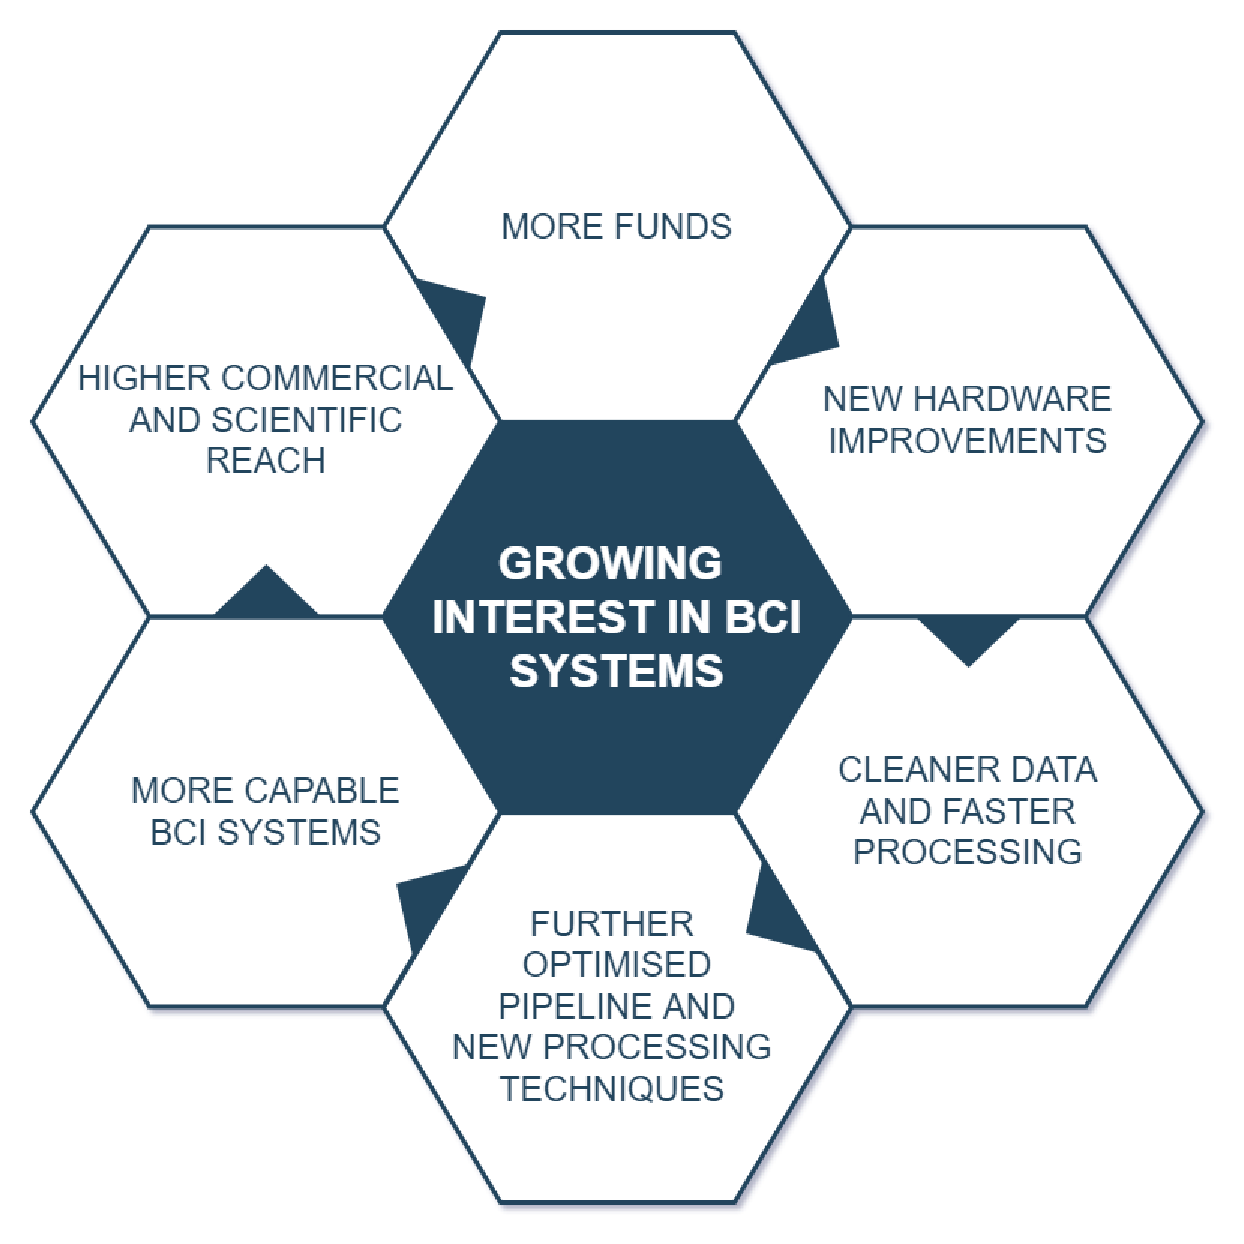
\includegraphics[width=0.7\linewidth]{../images/introduction/cyclic_interest_gain.pdf}
    \captionsetup{width=0.7\linewidth}
    \captionsetup{justification=centering}
    \caption{Summary of some of the potential reasons \gls{bci} research has seen its gain in popularity discussed in section \ref{sec:bci_gaining_popularity}. There is no clear chronological order for these events and they likely influence each other all at the same time.} 
    \label{fig:cyclic_popularity_increase}
\end{figure}

The potential reasons that were discussed can be separated into four major categories.
First, an increased interest by big-tech companies causes big funds to get into the field.
Secondly, improvements in measuring equipment allow for higher quality data and a more pleasant \glsfirst{ux}.
Third, processing equipment has seen increased affordability whilst also improving the computational power and portability allowing systems to be more affordable and capable.
Finally, more optimised software allows for better classification results and faster development of new systems.
It is highly unlikely all of these reasons have equal influence or that they are the only reasons for the improved popularity, but they should give the reader a better understanding of the context \glspl{bci} are currently in without becoming too technical.
The next section focuses on effective use cases for \glspl{bci} to let the reader understand the different capabilities of these systems even more.



% ---------------------------------------------- 
% USE CASES
% ---------------------------------------------- 

\section{Common use cases for BCIs}
\label{sec:bci_common_use_cases}

The previous section aimed to address potential reasons for the increase in popularity in \gls{bci} research.
This already discussed multiple \gls{bci} applications, showing some of the use-cases for \glspl{bci}.
When looking at Wolpaw's definition of a \gls{bci}, a \gls{bci} is nearly limitless in what it can be used for.
Whilst it should be a \textit{communication device}, this terminology can be seen rather broadly.
Most obvious is perhaps the use of a \gls{bci} as a control system, which then communicates with an external device so that it can be controlled.
Already discussed examples of this type include the multimedia control system proposed by \citet{early_bci_multimedia} from Section \ref{subsec:bci_gaining_popularity_better_processing}.
However, when using \glspl{bci} to detect common patterns of a disease, these patterns could also be communicated to a doctor and hence it could also be considered a communication device.
It should also be noted that the given definition of both a \gls{bci} and perfect \gls{bci} from section \ref{sec:bci_introduction} are around 20 and 10 years old respectively.
During the time that has passed since then, many new use cases for \glspl{bci} have emerged, especially in a commercial setting.
Thus, these definitions are by no mean the only definition for what a \gls{bci} system is and it is not uncommon to find varying opinions on what can be called a \gls{bci} system and what can't be called one.
This section aims to familiarize the reader with a broad idea of possible use cases of \glspl{bci} and to give some concrete examples whilst also addressing some of the shortcomings found in the articles describing them.
As this thesis focuses on non-invasive \gls{eeg} based \glspl{bci}, this section will also focus on non-invasive \gls{eeg} related articles.

For the interested reader, \citet{bci_review_arnau} provides more examples of \gls{bc} systems, of which \glspl{bci} are a subset, that use \gls{dl}.
The focus of \citet{bci_review_arnau} is on articles that provide at least a completely working \glsfirst{poc}, from live data acquisition to external device control.
\Citet{ml_strats_used_in_papers} reviews several \gls{bci} specific papers and focuses on the type of \gls{ml} task that is performed and which \gls{ml} and \gls{dl} techniques are used for this.
Only a few articles discussed by \citet{ml_strats_used_in_papers} have a working \gls{poc} on live data with many simply looking at the evaluation metrics of the \gls{ml} and \gls{dl} strategies.
Whilst the articles discussed by \citet{bci_review_arnau} are thus more representative of real-world performance and use-cases, finding such complete works is rather challenging.
Because this section is only meant to demonstrate potential use cases of \glspl{bci} and common shortcomings in the papers discussing them, there is no enforcement of requiring the discussed papers to have a fully working \gls{poc}.
This allows for offline systems and articles focusing on only certain components of the \gls{bci} pipeline to be discussed as well.
It also allows for discussing systems which may not strictly be \glspl{bci} but which do use almost identical pipelines, further demonstrating what is possible when working with brain signals as data.
In this regard, it is similar to the work of \citet{bci_applications} who give an overview of the most common use cases for \glspl{bci} and the challenges they are faced with.

% - - - - - - - - - -
% diseases
% - - - - - - - - - -

\subsection{Using BCIs as an automated tool in all stages of medical phenomena}
\label{subsec:bci_common_use_cases_medical_phenomena}

As \gls{eeg} is relatively affordable and portable, it is an often used modality in the hospital.
The visualisation of the measurements can be read by a specialist to diagnose a whole suite of diseases.
Especially seizure-related disorders such as epilepsy are often diagnosed through \gls{eeg} readouts \citep{eeg_epilepsy}.
Other neurological disorders such as the \gls{lis} can also be correctly identified by \gls{eeg} readouts \citep{eeg_lis_detection}.
Even the psychological field uses \gls{eeg} as a physiological measuring tool to aid in the diagnosis and psychological treatment of patients, although psychiatrists should be aware of the limitations \gls{eeg} has for them as further discussed by \citet{eeg_for_psychiatric}.
Since \gls{eeg} is used for a wide variety of diagnoses and by far the most common source of data for non-invasive \gls{bci} \citep[as discussed by][]{bci_review_arnau}, much research has gone into how \glspl{bci} can be used as an automated aid for medical diseases throughout all stages of a medical phenomena.
In general, three important distinctions are made for the stage of such phenomena and thus for the medical application of the \gls{bci}: prevention, diagnosis/monitoring and rehabilitation/restoration.

% | | | | | | | | | | | | |

\subsubsection{Using BCIs for the prevention of medical phenomena}
\label{subsubsec:bci_common_use_cases_medical_phenomena_prevention}

One popular example of prevention relates to the use of \gls{bci} systems for continuously monitoring signs of decreased attention \citep{bci_applications}.
Such a decrease in attention might show an exaggerated usage of alcohol and other drugs, which allows the user to be alerted before drinking \textit{just one more}.
Whilst it is unlikely that alcohol addicts will wear a \gls{bci} to the pub, such devices can significantly help in the reduction of traffic accidents by becoming mandatory during driving.
According to \citet{traffic_deaths}, traffic accidents were the number 1 cause of death for children and young adults.
Whilst many types of equipment are already in place to prevent traffic accidents from occurring, such as speed cameras and lane assist technology, it has been studied how \glspl{bci} can be used as a prevention measure as well.

Section \ref{subsec:bci_gaining_popularity_better_processing} discussed research by \citet{early_bci_drowsiness} as one of the first attempts to make a fully portable \gls{bci}.
As it measured drivers' drowsiness levels, the proposed system alerts or even enforces drivers to take a break from driving when drowsiness levels are too high.
Research such as that by \citet{eeg_dangerous_situation_car} has discovered that emergency situations in vehicles can be classified faster from \gls{eeg} data than the user's response, which could have a significant impact on reducing the number of traffic accidents.
\Citet{eeg_dangerous_situation_car} used a driving simulator to conduct a real-world experiment and they found that their proposed system has an accuracy of around 70\%.
One potential issue with this paper is the fact that their focus lies on this overall accuracy metric rather than providing the \textit{sensitivity} and \textit{specificity}.
Sensitivity could be seen as the accuracy of the model on positive cases (i.e. identifying a dangerous scenario as dangerous) whilst specificity denotes the accuracy on negative cases (i.e. identifying a non-dangerous scenario as non-dangerous).
However, \citet{eeg_dangerous_situation_car} do provide the \gls{roc} and provide reasoning for choosing an optimal classification threshold that resulted in this 70\% accuracy.
This threshold specifies how certain the classification prediction should be before acting on its classification.
This shows that it is important to look at more than just accuracy, as for this application being good at taking action in case a dangerous scenario is present is ideal, but taking action when there is no dangerous scenario could create a dangerous scenario itself.
Section \ref{subsec:processing_signals_general_pipeline_evaluating} discusses how to evaluate systems using different metrics and reasoning in more detail.
Many other examples of using \glspl{bci} for the detection of symptoms that can lead to traffic accidents exist. 
\Citet{eeg_motion_sickness} developed a system that could estimate motion sickness levels, which in turn could again be used to alert drivers to take a break.

The three discussed examples show how \glspl{bci} can be used in a variety of ways for the prevention of traffic accidents.
It also highlighted the importance of correct model evaluation and how a net benefit of a system is important.
For example, if the system proposed by \citet{eeg_dangerous_situation_car} would use the emergency brake each time it detects a dangerous scenario but has a poor specificity, it would heavily break in circumstances where it is not needed.
This in term creates risk if nearby drivers don't pay attention and cause a collision due to the abrupt emergency braking.
Thus, the question should be asked if a net benefit would be reached by those systems if the amount of prevented accidents outweighs the added risk of new accidents.
Likewise, it has to be considered if a \gls{bci} system is the most viable option, even if it has promising results.
Using a \gls{bci} to monitor if a driver is drunk and prohibiting him from driving if so might be more expensive and less efficient than \gls{baiid} which already exist.
Nonetheless, many applications exist for the prevention of traffic accidents and the prevention of other medical phenomena using \glspl{bci}, even if it is used as supplemental validation over existing devices and tests.
\citet{bci_applications} provides some extra examples of this type.

% | | | | | | | | | | | | |

\subsubsection{Using BCIs for the diagnosis and monitoring of medical phenomena}
\label{subsubsec:bci_common_use_cases_medical_phenomena_monitoring}

Section \ref{subsec:bci_gaining_popularity_improved_data_processing} already introduced the \glsfirst{cad} pipeline.
\gls{cad} systems, and the very similar \gls{cade} systems, using medical imagery are widely used for diagnosis and treatment monitoring in oncology and other fields.
Comparable systems exist using \gls{eeg} and other brain-signal measuring modalities for diagnosis medical phenomena and monitoring of the treatment.
The commercial Muse headset for sleep tracking that was discussed in Section \ref{subsec:bci_gaining_popularity_big_tech} is one example of a system that can be used for monitoring and diagnosing sleep patterns.

Whilst the Muse headset is a commercial product, medical \glspl{bci} exist which are made for detecting sleep patterns.
One very popular example is using \gls{eeg} for detecting sleep apnea, a medical sleep disorder.
\Citet{eeg_sleep_apnea} proposed an \gls{eeg} based \gls{bci} system for automating the detection of sleep apnea.
\Citet{eeg_sleep_apnea} named their used \gls{ml} approach \textit{Artificial Bee Colony Optimize Hermite Basis Functions}.
This paper is an example of a system that is highly specialized for a specific problem, namely detecting sleep apnea, requiring a lot of expert knowledge since it relies on a complex feature engineering step tailored towards detecting sleep apnea. 
Whilst this makes it unlikely the same pipeline can be used for the detection of other disorders, it does provide outstanding performance with a discussed sensitivity, specificity and accuracy of over 99\%.
The article by \citet{eeg_sleep_apnea} focuses on the \gls{ml} aspect of the proposed system, by re-using an existing dataset and describing only metrics related to the classification performance.
Since this system doesn't take specific control over an external device, it isn't a control system.
However, it could be argued it still communicates the detection of sleep apnea patterns and it can be deployed in a live system to alert a nurse when these patterns occur during a trial so that the nurse can pay additional attention during that period.
In this regard, naming the system proposed by \citet{eeg_sleep_apnea} a \gls{bci} is controversial, as is the case for most \gls{eeg} based systems that diagnose and monitor medical phenomena. 
Whilst \citet{eeg_sleep_apnea} don't mention the term \glsfirst{bci} in their article anywhere, in an article of a similar system, \citet{bci_sleep_apnea} do call their \gls{eeg} based detection of sleep apnea a \gls{bci}.

Many other types of diagnosis and monitoring can be done by non-invasive \gls{eeg} based \glspl{bci}.
The review article by \citet{bci_applications} addresses the detection of brain tumours \citep{eeg_brain_tumor1, eeg_brain_tumor2} and breast cancer \citep{eeg_breast_cancer}.
The review article by \citep{eeg_diagnosing_dyslexia} discusses the use of \glspl{bci} for the detection of dyslexia.
It should become apparent that many detection systems for medical phenomena can be made from non-invasive \gls{eeg} data. 
Even if these medical phenomena seem unrelated to the brain, such as for the detection of breast cancer \citep{eeg_breast_cancer}.
However, as these systems lack a true communication factor besides informing doctors or nurses, it can be argued if these systems are indeed \glspl{bci} w.r.t. Wolpaw's definition of a \gls{bci} given in Section \ref{sec:bci_introduction}.

% | | | | | | | | | | | | |

\subsubsection{Using BCIs for the rehabilitation and restoration after medical phenomena}
\label{subsubsec:bci_common_use_cases_medical_phenomena_restoration}

Restoration of lost mobility and rehabilitation is the third and final stage of most medical phenomena.
In this stage, a \gls{bci} can be of aid to both the medical staff and patient.
Out of the three discussed stages it is also the one that has seen the most \gls{bci} related research.
One reason for this is that many techniques for the restoration of lost mobility and rehabilitation rely on \gls{emg}, a modality used for measuring muscle-based \glspl{biosignal}.
Famous examples of such \gls{emg} based systems include prostheses which are connected to the remaining muscles of an amputated body part or an exoskeleton which is placed over body parts to strengthen their movement or re-enable them. 
Whilst in general \gls{emg} based systems far outperform \gls{eeg} based systems for prosthesis and exoskeletons, the \gls{emg} modality does not apply to patients suffering from an impaired neuromuscular system.
Thus, for these patients an \gls{eeg} based solution may offer them a possibility of regaining mobility again.
Since \gls{eeg} based \glspl{bci} for prosthesis and exoskeleton control are very common research in the \gls{bci} field, it will be discussed further in it's own section, Section \ref{subsec:bci_common_use_cases_prosthesis_exoskeleton}.

\Glspl{bci} have found their usage in other aspects of the rehabilitation and mobility restoration process as well.
In neurological rehabilitation, \glspl{bci} can function as a tool for guiding both patients and medical staff in what abnormalities are present in the brain and how they can be circumvented.
Intuitively, these \gls{bci} systems aim to improve the brain's ability to adapt itself based on experience.
This self-adapting property of the brain is known as brain plasticity or neuroplasticity.
A well-developed \gls{bci} system could show patients and medical staff which regions of the brain are currently being used and which types of brain signals and abnormalities are being detected.
This information could then be relayed to the patient through various means so that it induces neuroplasticity.
Such systems are still in development and require sophisticated neurological expertise that falls outside the scope of this master' thesis.
However, they are very promising and the interested reader is referred to the overview provided by \citet{bci_rehabilitation}.
It is noted once more this paper was co-authored by Professor Jonathan R. Wolpaw, which has been discussed in this paper multiple time for his definition of a \gls{bci} and a perfect \gls{bci}.

Another area that is often researched in the rehabilitation and restoration process, is using \glsfirst{mi} tasks to improve recovery of control over certain body parts.
The main idea behind such systems is to let the patient perform a \gls{mi} task, which doesn't require effective movement of the body part with reduced control.
This \gls{mi} task can then be classified by the \gls{bci} system based on the \gls{eeg} data and an exoskeleton is used to perform that motion as passive feedback.
Most commonly, a pedalling \gls{mi} task is used to control a motorized pedal, which evokes \gls{erd} patterns resulting in a greater potential for lower-limb recovery.
The works by \citet{pedal_mi_rehabilitation1} and \citet{pedal_mi_rehabilitation2} discuss such systems in greater detail.
Likewise, stroke rehabilitation and a reduction of the effects from the Parkinson's disease can be achieved with \gls{bci} guidance as well, as further discussed by \citet{parkinson_stroke_reduction}.

It is noted that many more \gls{bci} applications exist for preventing, monitoring and controlling diseases than those discussed here.
The work by \citet{bci_in_medicine} highlights some use-cases of \gls{bci} in medicine for example.

% - - - - - - - - - -
% prosthesis exoskeleton
% - - - - - - - - - -

\subsection{Using BCIs for prosthesis and exoskeleton control}
\label{subsec:bci_common_use_cases_prosthesis_exoskeleton}

Arguments were given why the medical applications of \gls{eeg} processing systems discussed in Section \ref{subsec:bci_common_use_cases_medical_phenomena} can or can't be considered \gls{bci} systems.
The main discussion revolves around the kind of communication that the system does.
To some authors, a system that alerts or visually informs medical staff based on processed data from \gls{eeg} can be considered a \gls{bci} system whilst others specifically expect an external device to perform a specific action based on the brain signals to name a system a \gls{bci} system.
The latter would be a type of control system, as the \gls{bci} controls an external device.
In a review article by \citet{bci_review_arnau}, it is found that among \gls{eeg} based \gls{bci} control systems using \gls{dl}, the control of robotic arms is most popular in research.
This section will discuss the use of \glspl{bci} as a control system for prostheses and exoskeletons.

% | | | | | | | | | | | | |

\subsubsection{Why BCIs are used for prosthesis and exoskeleton control}
\label{subsubsec:bci_common_use_cases_prosthesis_exoskeleton_why}

Most of the current robotic prostheses and exoskeletons rely on muscular activity in the body.
Just like brain activity can be measured by non-invasive \glsfirst{eeg}, muscular activity can be measured by non-invasive \glsfirst{emg}.
For example, patients who have had a partial loss of a body part often still have muscular activity in the remaining body part.
In the case of surgical amputation, the amputation is often done such that as much muscle remains to ensure as much possible muscular activity also remains.
These patients can then often still generate the muscular activity that would have been required for moving the missing body part.
This muscular activity can then easily be measured with the \gls{emg} modality, which is in general of higher signal quality than \gls{eeg} \citep{hybrid_eeg_emg_prosthesis}.
This \gls{emg} data can then be processed to classify the wanted movements and control robotic prostheses.
\Citet{emg_prosthetics} discuss the design and development of such a system based on \gls{emg} in greater detail.
Since the overall pipeline of such \gls{emg} based systems is quite comparable to the pipeline of \gls{eeg} based \glspl{bci}, many of the processing techniques are similar to those discussed in this thesis.
Alternatively, when the body part is still fully intact but the control over that part is lost or requires extra support, an exoskeleton may be used similarly.
Just like robotic prostheses, most exoskeletons rely on \gls{emg}.
A thesis by the German \citet{emg_exoskeleton} highlights the fundamentals of \gls{emg} based exoskeletons.

As was already touched upon in the rehabilitation and restoration part of Section \ref{subsec:bci_common_use_cases_medical_phenomena}, \gls{emg} measurements are not applicable for all patients.
In particular, people who have neurological diseases, limiting the production of the required muscular-based \glspl{biosignal}, fall outside the scope for these solutions.
However, the viability of robotic prostheses and exoskeletons for these patients has been steadily on the rise as \gls{eeg} based \glspl{bci} have been proposed for this purpose.
\Citet{bci_prostheses} give an in-depth systematic review of upper and lower limb exoskeletons and robotic prostheses controlled by \gls{eeg}-based \gls{bci}.
Just as was the case for rehabilitation and restoration discussed in Section \ref{subsec:bci_common_use_cases_medical_phenomena}, these systems often make use of brain signals measurable after imagined movement.
This process of thinking of movement but not doing the movement is known as \glsfirst{mi} and further discussed in Section \ref{subsec:biomedical_signals_brain_signals_measurable_brain_activity}.


% | | | | | | | | | | | | |

\subsubsection{The risk of using BCIs for prosthesis and exoskeleton control}
\label{subsubsec:bci_common_use_cases_prosthesis_exoskeleton_risk}

Whilst it is clear to see why \gls{eeg} based \glspl{bci} are promising for prosthesis and exoskeleton control from the discussion above, it should be noted that there is also a great risk in doing so.
\Citet{bci_prostheses} address the high risk associated with failed instructions for robotic prostheses and exoskeletons.
This means that the risks that can follow from misinterpreted instructions of exoskeletons and robotic prostheses are of such a degree that even high accuracy systems might not be good enough to guarantee a net benefit for the user.
This could be the reason that the review article by \citet{bci_review_arnau} didn't find any \glsfirst{poc} applications for exoskeleton or prosthesis control using \gls{eeg} based \glspl{bci}.
However, \citet{bci_review_arnau} did find many papers controlling an external robotic arm which is not connected to the body and thus not seen as a prosthesis.

\Citet{bci_prostheses} also highlight that whilst multi-label classification of \gls{eeg} is possible with considerable accuracy in an offline lab setting, the number of detectable classes is limited in a real-time and real-life environment.
Because of this, \gls{eeg}-based systems in these applications still have some challenges to overcome to match the precision and reliability of \gls{emg} counterparts.
Whilst improvements regarding these aspects have been made since the work of \citet{bci_prostheses} was published, the main challenges remain to this day, especially when using affordable systems.
Because of this, widespread adoption of \gls{eeg}-based exoskeletons and robotic prostheses is still very limited.


% | | | | | | | | | | | | |

\subsubsection{Promising steps towards BCI controlled prosthesis and exoskeleton control}
\label{subsubsec:bci_common_use_cases_prosthesis_exoskeleton_promosing_steps}

Whilst the discussed risk has caused widespread adoption of \gls{eeg}-based exoskeletons and robotic prostheses to still be very limited, promising steps are being made to bring them to market.
These systems mainly focus on robotic arms, which are not strictly a prosthesis but they pave the road to \gls{bci} controlled arm prosthesis in the future.
These proposed systems often rely on incorporating supplementary information such that risky movements are cancelled, even if the \gls{bci} requests them. 
\Citet{bci_mi_robotic_arm_collision_avoidance} proposed such a system to control a robotic arm not only through a \gls{eeg} based \gls{bci} working with \gls{mi} tasks but also by using obstacle avoidance algorithms to reduce the risk of harmful contact, computer vision for object detection to get a better idea on the possibly wanted interaction and eye-tracking to gather extra information surrounding the user's intention.
Other successful research on making more reliable \gls{bci} systems for controlling robotic arms is done by \citet{eeg_robot_arm1, eeg_robot_arm2, eeg_robot_arm3, eeg_robot_arm4}, these articles are also included in the review article on \gls{dl} based \gls{bc} systems by \citet{bci_review_arnau}.

Whilst limb prostheses, currently being pilot run through robotic arm research, are one of the most common and researched types of prostheses, they are only a fraction of all prostheses in existence.
Everything from dentures to artificial breasts can also be labelled as a type of prostheses.
For example, visual prostheses such as bionic eyes are another type of prostheses that has active research in the \gls{bci} field.
Not only can \gls{bci} systems improve visual prostheses, many of the existing visual prostheses could be seen as a special type of \gls{bci} system as a whole.
Both the works by \citet{bci_blind_assist_review} and \citet{bci_vision_assist_review} give an overview on the progress in visual prostheses in the \gls{bci} field.
These \glspl{bci} are often invasive and opposed to only reading brain activity, they can also stimulate the brain and other parts of the body.
Through this stimulation or by other means, the user can regain some form of vision from these \gls{bci} systems.
Second Sight is one of few companies that has commercially made visual prostheses with approval from the \gls{fda}.
Their system is discussed in the overview on \gls{bci}-related vision restoration systems by \citet{bci_vision_assist_review}.
The international trial by \citet{second_sight_trial} on the products of Second Sight shows promising results, although it is noted the study is performed by Second Sight employees and not by an independent research team.
The exact working of visual prostheses or, more specifically, Second Sight products is not of interest for this work, but the recent decisions of Second Sight company reveal one of the largest risks of invasive \glspl{bci} and \glspl{bci} in general.
Due to the discontinuation of some of the Second Sight products, hundreds of users are left without product support for a system that shaped their everyday life.
Besides this, the now non-functioning product is still present inside their body.
The issues and ethical questions this brings to the table are discussed further in Section \ref{subsec:bci_ethical_e_waste}.


In summary, hybrid systems like the one by \citet{bci_mi_robotic_arm_collision_avoidance} are very promising as they can greatly reduce the risk involved in many \gls{bci} systems, such as prostheses-related applications, whilst also increasing the overall accuracy of the system.
Section \ref{subsec:bci_common_use_cases_improving_existing_system} discusses more of these hybrid systems but where \glspl{bci} are used as supplementary component to an existing system.


% - - - - - - - - - -
% improving system
% - - - - - - - - - -

\subsection{Using BCIs to improve the working of existing systems}
\label{subsec:bci_common_use_cases_improving_existing_system}

The previous sections discussed the use of \glspl{bci} as a control system for prostheses and exoskeletons.
Whilst this approach was promising for certain patients, the high risk associated with such systems meant that developing reliable systems relying solely on \gls{eeg} based \glspl{bci} was not yet possible \citep{bci_prostheses}.
One area that did see success was the use of \textit{hybrid \glspl{bci}} as a control system for robotic arms.
Such hybrid systems combines \gls{bci} techniques with other techniques to create an overall system that is more accurate, safe and reliable and thus complies more with Wolpaw's definition of a perfect \gls{bci}.

The discussed hybrid systems from Section \ref{subsec:bci_common_use_cases_prosthesis_exoskeleton} considered the \gls{bci} as the main component with the other techniques, such as computer vision, added as support and improvement to it.
There are also multiple examples of where a \gls{bci} system is added as an \textit{extra component} to an existing system and thus not considered the main component.
This allows for \glspl{bci} to find use cases in non-trivial domains.
To demonstrate this, an extension to classical hearing aids using an \gls{eeg} based non-invasive \gls{bci} is discussed in this section.
This section also addresses the use of \glspl{bci} to make \textit{smart homes} more accessible for people with a handicap and the elderly.
It also addresses some other examples of hybrid \glspl{bci}.


% | | | | | | | | | | | | |

\subsubsection{Extending hearing aid systems with BCIs}
\label{subsubsec:bci_common_use_cases_improving_existing_system_hearing_aids}

According to \citet{hearing_aids_noise_reduction} over 450 million people suffer from disabling hearing loss.
Most solutions to hearing loss rely on a microphone to capture environment audio which is then amplified and played through a speaker that is placed in or near the ear.
Most commonly, the microphones used for amplification are integrated inside the speakers that are placed in the ear to form a stereo setup that mimics regular hearing.
This is not always ideal when there is a lot of ambient noise.
Sometimes using an external directional microphone placed closer to the audio source of interest can form a solution.
For example, placing a microphone on the desk of a professor teaching in a noisy room of students.
However, this solution is not applicable in all situations.
Thus, most hearing aids include some noise suppression on the microphones directly to filter out ambient noise and amplify noise coming from human speech.
\Citet{hearing_aids_noise_reduction_mandarin} evaluated such noise suppression for Mandarin-speaking users and found the results to be good but not ideal, as there is a lot of variation in human speech tone making it hard to detect what is and what isn't ambient noise.

Even when such a noise suppressing filter would work optimally, people with hearing aids often still have trouble understanding people when multiple speakers are close-by at once.
Recent research by \citet{bci_hearing_aid_direction} has shown that using a non-invasive \gls{eeg} based \gls{bci} can improve traditional hearing aids in solving this problem.
\Citet{bci_hearing_aid_direction} does this by determining which speaker a user is listening to by analysing directional queues from the measured brain-signals.
If this information would be communicated to the hearing aids, it can allow them to optimize the microphones to pick up speech from that area only, filtering out other speakers.
Whilst great in theory, \citet{bci_hearing_aid_direction} discuss how a long waiting time to determine the area of interest challenges the practical usability of their system as of now.
Nonetheless, it shows one of many non-trivial ways a \gls{bci} could be used as an extension of existing systems to improve them.



% | | | | | | | | | | | | |

\subsubsection{Using BCIs to improve accessibility of existing applications}
\label{subsubsec:bci_common_use_cases_improving_existing_system_improve_accessibility}

There are still a lot of applications which lack support for people with disabilities or people with less technical skills.
Take for example the growing ecosystem of smart home applications, since it aims to automate many tasks such people might find difficult or impossible to perform, it can be very beneficial to these people.
However, conventional interaction methods are app-like through touch screens mounted all around the house.
Such interaction methods are not fit for people with limited movement capabilities or technical knowledge.

Since \gls{eeg} based \glspl{bci} are known to work well for conscious people that can learn how to effectively do \glsfirst{mi} tasks, it is often seen as a solution to provide novel interaction method with existing applications to improve accessibility.
\Citet{bci_smart_home_app} were one of the first to explore the idea of using a \gls{bci} for smart home control as they believed it could greatly improve the quality of life for the elderly and people with a handicap.
They used the Emotiv EPOC headset as a non-invasive source for the \gls{eeg} using dry electrodes and achieved high accuracy results through a primitive binary selection interface.
This means that it seems to comply with most properties of Wolpaw's definition for a perfect \gls{bci} except for one of the most important ones, it is not at all as fast as the regular interaction method.
Adding to this, their system doesn't make use of actual brain signals but rather relies on muscular activity, such as smirks and eyebrow movement.
This movement of the facial muscles is known to provide an easily detectable artefact in the \gls{eeg} and is often used as a supplementary input for the \gls{bci} system.
As section \ref{subsec:biomedical_signals_measuring_artefacts} will discuss in greater detail, such an approach has many negatives.
Finally, the system of \citet{bci_smart_home_app} was tested on four subjects but the article fails to deliver exact details on this experiment and it is assumed the participants were neither elderly nor people with a handicap.

Whilst this means the system by \citet{bci_smart_home_app} isn't a true \glsfirst{bci} due to the use of \gls{eeg} artefacts and the paper has questionable scientific value, it was one of the first to explore the idea of using a \gls{bci} for smart home control.
Since then, more articles have studied this idea using effective brain signals.
\Citet{feasibility_bci_smart_home} discuss this in their feasibility study about using \glspl{bci} for smart home control.
The article by \citet{feasibility_bci_smart_home} does include clear details on the experiment setup which includes two people with a handicap among 12 other healthy subjects.
It was found that the people with a handicap had an 81\% average accuracy whilst the healthy subjects only had a 77\% average accuracy.
Due to the low sample size, this difference in results is likely not statistically significant but these accuracy numbers are usable when taking into account the small risk of failed actions in basic smart home control systems.

% | | | | | | | | | | | | |

\subsubsection{Other examples of hybrid BCIs}
\label{subsubsec:bci_common_use_cases_improving_existing_system_smart_home}

Section \ref{subsec:bci_common_use_cases_prosthesis_exoskeleton} already discussed the use of a hybrid \gls{bci} system where computer vision, eye tracking and other technologies were used in combination with a \gls{bci} system to create a more reliable and accurate final system for robotic arm control \citep[as proposed by][]{bci_mi_robotic_arm_collision_avoidance}.
With existing algorithms such as the real-time grasp detection algorithm, GraspNet, by \citet{graspnet} for low-powered devices, it is very easy to envision how they can be used to improve a \gls{bci} related system.
Articles which propose a fully working \gls{poc}, such as the ones reviewed by \citet{bci_review_arnau}, often require these additional algorithms to ensure safe working in real-world environments.

One very interesting hybrid solution is the use of a non-invasive \gls{eeg} based \gls{bci} system with measurements from non-invasive \gls{emg}.
\Citet{hybrid_eeg_emg_prosthesis} proposed such a hybrid \gls{eeg}-\gls{emg} system for upper limb prosthesis control.
Since \gls{emg} is known to be a more accurate modality for prosthesis control, the system by \citet{hybrid_eeg_emg_prosthesis} uses \gls{emg} for movement of the prosthesis where possible and supplements it with \gls{eeg} data for determining the other wanted movements.
In particular, the proposed prosthesis by \citet{hybrid_eeg_emg_prosthesis} uses \gls{emg} present in the remaining upper arm muscles for elbow motion and \gls{eeg} for determining the desired wrist, grip and finger
motions.
The \gls{emg} part, which also imposes the greatest risk, had an accuracy of over 90\% whilst the \gls{eeg} part has an accuracy of over 65\%.

The combination of \gls{eeg} and \gls{emg} can also be used for other purposes.
\citet{thesis_arnau} proposed the use of both \gls{emg} and \gls{eeg} data for training a classifier which then relies solely on \gls{eeg} input for making final classification predictions.
Since the number of combinations to create hybrid \gls{bci} systems are nearly endless, it is left to the reader's imagination to come up with other potential use cases.

% - - - - - - - - - -
% P300 vs eye tracking
% - - - - - - - - - -

\subsection{Using BCIs as an alternative for eye tracking}
\label{subsec:bci_common_use_cases_bcis_replace_eye_tracking}

\gls{bci} systems relying on P300 signals where already briefly mentioned in Section \ref{subsec:bci_gaining_popularity_better_processing}.
As further discussed in section \ref{subsec:biomedical_signals_brain_signals_measurable_brain_activity}, a P300 signal is a positive bio-electrical wave measurable with \gls{eeg} around 300ms after a specific stimulus occurred.
This specific stimulus consists of a rare and contrasting stimulus when the user was focusing on what is otherwise a relatively static object with a frequent stimulus \citep{eye_tracking_vs_p300_comparable}.
The most famous example is the use of a computer screen showing elements in a grid-like pattern as the static object with a frequent stimulus and flashing one specific element as the rare and contrasting stimulus.
If the element the user was focused on flashes, the P300 signal will be present and relatively easily detectable in non-invasive \gls{eeg} measures.
A clever design of the interface can enable a wide variety of \gls{bci} applications.
This section will highlight a few of these applications.
It is noted that other types of stimulus can be used, such as auditory ones, to evoke a P300 signal.
However, this section focuses on the discussed, visual, grid-based methodology.

With such visual P300 based \gls{bci} relying on the before-mentioned method of focusing on a part of the screen and using flashing patterns to recognise which part the user is focused on, a viable alternative would be eye-tracking technology.
This makes the effective use of these types of \gls{bci} systems debatable, an issue that is also further discussed in this section.

% | | | | | | | | | | | | |

\subsubsection{Why a low learning curve makes P300-based BCI systems attractive}
\label{subsubsec:bci_common_use_cases_bcis_replace_eye_tracking_why_p300}

In general, \glspl{bci} using the P300 signal are often used as they have a low learning curve and there is a relatively low variation in performance between users compared to other types of \glspl{bci} \citep{p300_spellers, p300_spellers_review}.
The reason these systems have a low learning curve is due to their simple user interface and a combination of a system that generalises well and that has been studied thoroughly for the use of \glsfirst{tl}.
Early examples of using \gls{tl} for P300 related \glspl{bci} include those by \citet{p300_speller_tl}.
Adding to this, P300 signals can be detected with non-invasive \gls{eeg} using dry electrodes, which are available in multiple \gls{eeg} measuring headsets at affordable prices in a comfortable and visually pleasing package, as further discussed in Section \ref{subsec:biomedical_signals_measuring_equipment}.
Whilst these factors hint that such \gls{bci} systems comply with Wolpaw's definition for a perfect \gls{bci} addressed in Section \ref{sec:bci_introduction}, it will become clear in this section that the communication rate of these systems is still a limiting factor.

However, these aspects do make it possible for P300-based \glspl{bci} to be rapidly configured and used by a new user.
All of this aids in creating a pleasant \glsfirst{ux} even if the communication rate is low, as shown by user studies such as the one by \citet{p300_speller_real_life2}.
Other types of \gls{bci} systems, such as those relying on \Glsfirst{mi}, can have a tedious training procedure in advance.
This can cause psychological burden and other side effects for the user.
This gives rise to multiple ethical challenges, some of which are discussed in Section \ref{sec:bci_ethical}.
Considering these things, P300 based \glspl{bci} are an interesting choice as a \textit{first \gls{bci}} to introduce the user to the possibilities of \gls{bci} systems.
This might make it easier for the user to move to a more capable and sophisticated system that has a steeper learning curve, higher cost and more demanding training.

Research on the \gls{ux} is often overlooked by initial \gls{bci} system proposals, where the focus is often on objective numerical measures such as speed, accuracy, sensitivity and specificity.
However, as discussed by \citet{thesis_arnau}, user studies are essential to even consider using a proposed \gls{bci} system in the real world.

% | | | | | | | | | | | | |

\subsubsection{Using BCIs for P300 spellers}
\label{subsubsec:bci_common_use_cases_bcis_replace_eye_tracking_p300_spellers}

By far the most common usage of the P300 signal is to create \textit{p300 spellers}, an idea first described by \citet{first_p300_speller}.
In its simplest form, P300 spellers simply show the alphabet as grid elements and let the user spell words letter-by-letter.
More complex forms can use auto-correction to correct faulty classifications, reducing the effective error of the system.
Advanced text prediction can also be used to show complete words or sentences for selection, increasing the communication rate as opposed to letter-by-letter input.
Other techniques can also further increase the reliability and communication rate of the system.

As such, P300 spellers are examples of novel interaction methods that aim to replace keyboards for those who don't have the required capabilities to operate them.
Especially patients with severely limited motor skills and communication capabilities such as people suffering from serious cases of \gls{als} or \glsfirst{lis} can benefit from these systems by regaining basic communication skills \citep{p300_spellers, p300_spellers_review}.
Whilst wrong classifications in a speller application could result in unpleasant situations, it is clear that the risk involved is far smaller than with \gls{bci} system used for controlling prostheses and exoskeletons such as discussed in Section \ref{subsec:bci_common_use_cases_prosthesis_exoskeleton}.
This makes P300 spellers one of the few types of \gls{bci} systems that are actively being used in the real world.

\Citet{p300_speller_real_life} performed a usability study of P300 spellers with 20 \gls{als} patients in a real-life environment.
According to \citet{p300_speller_real_life}, most participants achieved over 70\% accuracy, which is in line with the findings of \citet{p300_spellers_review} and \citet{p300_speller_real_life2} in similar studies amongst other types of patients.
More interestingly, even though the accuracy wasn't extremely high, all participants of the experiment by \citet{p300_speller_real_life} succeeded in the given tasks.
This is in part due to our ability as a human to understand typo's in words and sentences relatively easily.
Another important factor is that the studied system makes use of the earlier discussed auto-correction and text-prediction techniques.
Whilst far from advanced variants of these techniques were used, it almost doubled the communication rate of the P300 speller already with the mean number of correct symbols per minute going from 3.6 to just over 5.

Whilst 5 symbols per minute is significantly slower compared to traditional communication skills, it enables useful communication for those who can't communicate through regular means.
It should also be considered that these results are for people suffering from \gls{als}.
These people can have difficulties with controlled eye movement or rapid eye movement which results in a slower operation speed compared to able-bodied persons.
However, since it is so slow compared to the regular interaction method of able-bodied persons, it is far from a perfect \gls{bci} when taking into account Wolpaw's definition of a perfect \gls{bci}.
A similar study by \citet{p300_speller_real_life2} focuses more on the \gls{ux} for \gls{dmd} patients using P300 spellers.
This study has shown that P300 spellers can be used by \gls{dmd} patients with satisfactory results in a pleasant manner for the user, even if the communication rate is slow.

% | | | | | | | | | | | | |

% TODO; hieronder verder lezen, reeds spell checked etc

\subsubsection{Using the P300 signal for other BCI applications}
\label{subsubsec:bci_common_use_cases_bcis_replace_eye_tracking_p300_other_applications}

When taking a broader look at P300-based \gls{bci} systems using a visual grid system, they are just a mechanism for recognising which portion of the screen a user is looking at.
These grids are often of a limited size, such as 6 by 6, for the best trade-off between accuracy and communication rate.
The effective content of the grid and the actions taken upon classification can vary widely.
This has enabled the exact technology of P300 spellers to be easily adapted for other applications.

One such example is the \textit{Facebrain} application by \citet{facebrain}.
Facebrain provides a non-invasive \gls{eeg} based \gls{bci} for interacting with the social media platform Facebook.
In essence, it's a regular P300 speller with the first screen(s) representing possible actions to take on the platform.
When text input is required, a regular P300 speller user interface is presented.
This allows a user to operate almost all of Facebook's functionalities with only a P300-based \gls{bci}.
The application by \citet{facebrain} is one of many that shows the same strategy and classification algorithms as P300 spellers can be used for a wide variety of applications by changing the meaning and functionalities of the shown grid elements.
Rather than showing symbols, a complete image could be shown and separated into grid elements as well.
\Citet{p300_drone} used this idea by showing a live video stream from a quad-copter and moving it towards where the user is looking based on the P300 signal after flashing different portions of the image.
However, as the video live stream is not static, the contrast between the flash and regular screen content shrinks making the P300 signal less noticeable and thus the classification task harder.

% | | | | | | | | | | | | |

\subsubsection{Why eye tracking may still be preferred}
\label{subsubsec:bci_common_use_cases_bcis_replace_eye_tracking_eye_tracking_better}

Whilst the discussed P300 applications have shown success in achieving their goals, the effective real-world use of such systems can still be debated.
The communication rate is slow and for able-bodied users, traditional eye-tracking can far outperform these systems \citep{eye_tracking_vs_p300_comparable}.
Adding to this, as P300 signals are a type of \gls{erp}, there are some known limitations and issues with techniques relying on them as well.
The \gls{bci} handbook by \citet[Chapter~26]{bci_handbook} discusses the crowding effect, adjacency problem, repetition blindness and user discomfort amongst other issues \glspl{erp} have.
Most of these problems arise from the often limited space for sending visual stimuli without overlap and the changing behaviour of both the brain and participant's experience after a prolonged session where many stimuli have been applied.

Multiple articles have been written on when and why a P300-based \gls{bci} might be preferred over a regular eye-tracking system \citep{eye_tracking_vs_p300_comparable, p300_eyetracking_slower}.
The experiments performed by \citet{eye_tracking_vs_p300_comparable} compared the accuracy and communication rate of visual P300 based \glspl{bci} against traditional eye-tracking solutions.
\Citet{eye_tracking_vs_p300_comparable} found the accuracy of both systems to be comparable but the communication rate of eye tracking solutions was around 50\% faster.
However, when questioning the ten participants of the study, it was found that there is a higher preference for the \gls{bci} system than the eye-tracker.
Whilst favourable for the \gls{bci} alternative, the results of the study by \citet{eye_tracking_vs_p300_comparable} should be interpreted with caution.
The participants of their study were all able-bodied persons and the eye-tracking experiments were always performed last.
This and other aspects of their methodology are bound to introduce bias in the results.

A study by \citet{no_interest_in_using_p300} compared the use of eye-tracking software and auditory P300 based \glspl{bci} for a patient suffering form the \glsfirst{lis}.
Whilst the patient was able to work with both systems autonomously, there was a strong preference for the traditional communication strategy which relied on a human to determine the wanted communication of the patient.
This preference was purely based on the \gls{ux} rather than the communication rate.
Whilst only being an experiment based on a singular participant, it does show how automated systems for regaining basic communication might cause a negative psychological impact on the user.
Thus, the results found by \citet{eye_tracking_vs_p300_comparable} on \gls{ux} are in direct contrast with the results from the experiment by \citet{no_interest_in_using_p300}.
However, \citet{no_interest_in_using_p300} lacked a study of visual P300 based \glspl{bci}, so it could be that such a system would be preferred. 

Similar conflicting results are present on other aspects of visual P300 based \glspl{bci} as well.
One debate that has been active for years is the dependence of P300-based \glspl{bci} on the capability of a user to look directly to a single target for a prolonged time.
As discussed by \citet{p300_eye_gaze}, it has been argued that this dependence is low as peripheral vision allows the user to focus on the desired element even if the eyes aren't directly rotated towards the element.
This would be favourable for P300 solutions compared to eye-tracking solutions as some users might not have the required muscle control to point their eyes to a specific point for prolonged periods, a task known as eye gazing.
However, the study by \citet{p300_eye_gaze} does show a dependence of P300-based systems on eye gaze and they argue the effective uses of visual P300 systems should be reconsidered.
Yet, the review article by \citet{bci_eye_gaze} addresses multiple articles which concluded through real-world tests that being capable of eye gazing is not necessary for effective use of P300-based \glspl{bci}.

These contradicting results on the use of P300-based \gls{bci} applications make it hard to determine which kind of system would be usable in the real world, providing a net benefit for the user.
It also shows that promising objective results such as a high accuracy and communication rate are not guaranteed to provide a system which is enjoyed by the end user.
Thus, many proposed systems require follow-up articles focusing on performing in-depth real-world experiments with the target population to conclude if they are worthwhile.
However, doing such a study in the same article proposing the new novel system would mean that one singular article takes an incredible amount of time.
This is contradictory to the expectations of many researchers in the field to publish a certain amount of articles yearly.
However, the latter is an ethical dilemma that entails a higher risk of \textit{sloppy science}.

% - - - - - - - - - -
% other use cases and summary
% - - - - - - - - - -

\subsection{Summary on the use cases for BCIs}
\label{subsec:bci_common_use_summary}


Since \glspl{bci} can be seen as a novel interaction method for controlling external devices, the possible use-cases are endless.
Even for the discussed P300 based \gls{bci} systems alone, a huge variety of applications can be created as addressed in Section \ref{subsec:bci_common_use_cases_bcis_replace_eye_tracking}.
This has caused review articles to focus solely on these types of \gls{bci} systems or even subset of those types of systems \citep{p300_review_article1, p300_review_article2, p300_review_article3}.

Thus, addressing all possible use cases for \glspl{bci} is far outside the scope of this thesis.
For this section, the goal was for the reader to obtain a more general insight into the most studied uses for \glspl{bci}.
In this regard, it succeeded in addressing all of the most popular use cases of \glspl{bci} as \gls{bc} systems in the real world as found by \citet{bci_review_arnau} and the most interesting use cases of \glspl{bci} addressed in the review article by \citet{bci_applications}.
It also highlighted that current real-world applications still rely on other technologies to limit risk and improve accuracy as standalone non-invasive \gls{eeg} based \glspl{bci} are still not accurate and reliable enough for most real-world usage.
Some of the main positive and negative points of the discussed articles were also addressed.

Most notable from this section is the fact that objective measures are only a small part of making a system that can be used in the real world.
Take for example the discussed experiment by \citet{p300_speller_real_life} which studied the use of P300 spellers by patients suffering from \gls{als}.
With a classification accuracy of 70\% and only 5 symbols per minute, the objective measures from this system look terrible compared to able-bodied alternatives such as regular keyboard typing.
However, \citet{p300_speller_real_life} found the users to have enjoyed the use of the P300 spellers and when taking into account the options available to the target users rather than able-bodied users, the objective measures are far more impressive.

However, even the articles which perform experiments that take into account the \glsfirst{ux} can sometimes cause conflicting results.
Take for example the discussed differences between the found user experience of P300 based \glspl{bci} between the experiment by \citet{eye_tracking_vs_p300_comparable} and \citet{no_interest_in_using_p300}.
Able-bodied persons from the experiment by \citet{eye_tracking_vs_p300_comparable} mentioned a pleasant \gls{ux}.
A more representative real-world study by \citet{no_interest_in_using_p300}, who looked at a singular patient suffering from \gls{lis} showed that this person had no interest in using such systems as a replacement for the existing human-based communication system which was already present.
Even-though speed and autonomous use were far better and the \gls{ux} according to the able-bodied persons was great, the \gls{ux} for this person suffering from \gls{lis} was not good enough.
Thus, the \gls{ux} is something that can only truly be measured when performing the experiments for an extended period with the target audience of the system, not through a single experiment on able-bodied participants.
It is hard for an able-bodied person to understand that the confrontational aspect of \glspl{bci} on the limitation a user has can outweigh the benefits it seemingly offers.
This and other more ethical questions are also addressed in Section \ref{sec:bci_ethical}.

To summarize, as a \gls{bci} performs actions based on brain signals, a very fitting analogy could be made: \textit{a \gls{bci} could do anything you can think of}.
That is, of course, only true in theory.
Due to limited knowledge of the brain \citep{brainmapping} and limitations in what can be measured, a \gls{bci} can only truly do what you can think of in a \textit{measurable way}.
Still, this is a whole lot of applications and an overview diagram of the most important ones is given in Figure \ref{fig:bci_use_cases_diagram}.
This diagram is not only based on the use cases discussed in this thesis but also those discussed in the articles by \citet{bci_review_arnau} and \citet{bci_applications} among others \citep{bci_review_book_chapter, bci_review, bci_in_medicine, bci_history, bci_review_monkey, bci_handbook}.
From Figure \ref{fig:bci_use_cases_diagram}, it should become apparent that most short-term goals of \glspl{bci} still lie in improving the quality of life for people with disabilities.
However, the rise in popularity of \glspl{bci} in the gaming industry and amongst other big tech companies, as discussed in Section \ref{subsec:bci_gaining_popularity_big_tech}, shows there is a potential future where \glspl{bci} find more real-life use-cases in other fields as well.

% TODO: overview based on review arnau en bci_applications, met die van bci_applications voorbeeld figuur
\begin{figure}[ht]
    \centering
    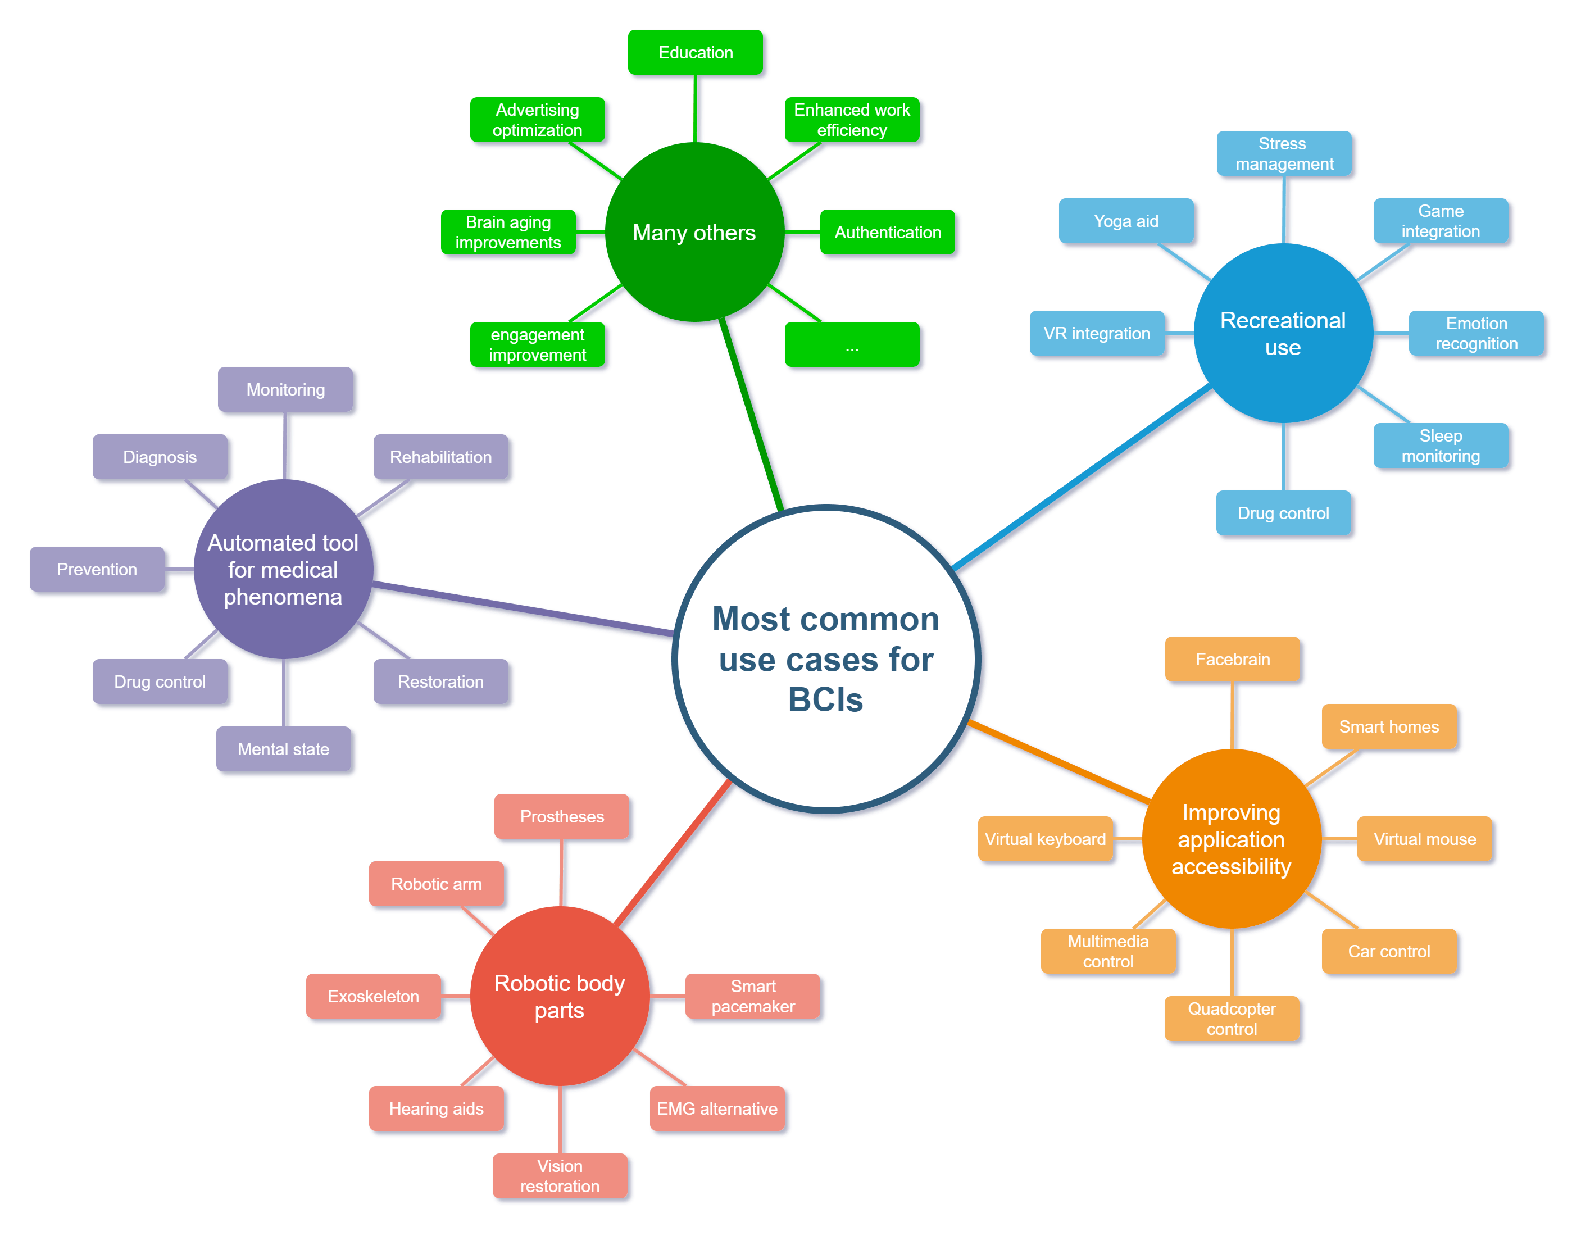
\includegraphics[width=\linewidth]{../images/introduction/use_cases_overview.pdf}
    \captionsetup{width=0.7\linewidth}
    \captionsetup{justification=centering}
    \caption{An overview of some of the many use cases for \glspl{bci}.} 
    \label{fig:bci_use_cases_diagram}
\end{figure}


% ---------------------------------------------- 
% Opportunities and obstacles for BCI research
% ---------------------------------------------- 

\section{Opportunities and obstacles for BCI research}
\label{sec:bci_opportunities_obstacles}

The most likely factors of why \glspl{bci} are gaining popularity and what the most common use cases are for \glspl{bci} were already discussed in Section \ref{sec:bci_gaining_popularity} and \ref{sec:bci_common_use_cases} respectively.
From these sections, an interested reader could have already spotted some opportunities and potential obstacles for doing research in the field themselves.
This section discusses some opportunities and obstacles present according to the author of this paper.
The aspects that are covered in this section are oriented towards the interests of the author from this master's thesis and aim to explain why this master's thesis came to fruition.
They also lay the foundation to the proposed \gls{bci} \gls{bc} system of this master' thesis, which will be further discussed in Section \ref{sec:bci_concolusion_and_proposing_ours}.


% ---------------------------------------------- 
% Small projects
% ---------------------------------------------- 

\subsection{Seemingly small projects with huge impact}
\label{subsec:bci_opportunities_obstacles_small_projects}

As \glspl{bci} and other technologies become more commercially oriented, the main focus is often shifted to providing products that can be used by the masses to provide the highest possible revenue.
Whilst \gls{bci} research sees its foundation from the medical world and most of the current users are people with a certain medical condition, a similar shift is likely, especially for the larger projects funded by big-tech companies.
This isn't necessarily a bad thing for medical applications, since this doesn't mean academic research focusing on those people with a certain medical condition disappears, rather it becomes a smaller portion of all research in the field.
The new technology and knowledge commercial products deliver can directly contribute to academic research focusing on medical applications.
This may include cheaper and more capable measuring equipment, a more socially acceptable picture of \glspl{bci} aiding the aesthetic aspect of Wolpaw's definition for a perfect \gls{bci} and better performing classification algorithms.
It is also possible that a commercial \gls{bci} application which is meant as a novelty for most, is life-changing to some.

Take the evolution of live captions as a recent example from a different domain, it has found its way directly into the Android smartphone operating system.
Whilst initially implemented for users to enjoy video content in situations where they can't listen to the audio, people with hearing difficulties now have a direct way to enjoy more content too.
The push for autonomous cars will allow those that are traditionally unable to drive a car to finally enjoy the freedom a car can offer as well without being dependent on others to do so.
Object and scene recognition algorithms made for optimizing smartphone cameras can also be used as a way of describing what is on a photograph for those who have limited vision.

Likewise, as more people are exposed to complex medical and commercial applications, many individuals start to envision seemingly small applications that could have a major impact on them or people they know.
This has been the case with smartphone applications for a long time.
A colour picker app that uses the camera to describe the colour of the central pixel is something that can be implemented with very limited resources.
Yet, such an application has already proven to significantly aid people who have colour blindness.
For example, they may use this application to determine whether a banana is ripe or not, something they can't visually determine but is easy with a textual description of the colour.
For such small applications to be feasible, an abundance of open-source material to re-use existing code for operating the camera, getting a textual colour description of an RGB colour code and more is required.

This presence of open-source code has started to emerge for the \gls{bci} field as well, as discussed in Section \ref{subsec:bci_gaining_popularity_better_processing}.
Combined with publicly available \gls{eeg} dataset such as the one by \citet{eeg_data}, it has become possible for developers to work on a pipeline without needing the monetary investment in \gls{eeg} measuring equipment.
If desired, the affordable headsets by OpenBCI and others, further compared in Section \ref{subsec:biomedical_signals_measuring_equipment}, make it possible to have \gls{eeg} measuring equipment with good open-source libraries for well under 1000 euros.
This has made individuals such as the author of this paper excited to create a wide variety of smaller applications that could have impactful meaning to some very specific people.
Especially the possibility of regaining even the simplest form of mobility through some very basic controls derived from \glsfirst{mi} is what motivated the author of this master's thesis to study the field.


% - - - - - - - - - -
% motivating aspects
% - - - - - - - - - -

\subsection{Motivational aspects for this master's thesis}
\label{subsec:bci_opportunities_obstacles_motivating_examples} 

The discussed use cases from Section \ref{sec:bci_common_use_cases} were motivating examples for this master's thesis in themselves.
However, there are some specific articles and aspects from the field that have motivated the creation of this master's thesis which will be discussed in detail here.
These are mainly related to \glsfirst{mi} based \glspl{bci} working with affordable consumer-grade and non-invasive \gls{eeg} measuring equipment.
Whilst many articles have demonstrated the potential of such \gls{bci} systems, the lack of widespread adoption suggests there are still hurdles to overcome for them to become a reality.
When discussing these motivating examples, some of these hurdles will already be discussed, the main obstacles for \gls{bci} research are further discussed in later subsections.


% | | | | | | | | | | | | |

\subsubsection{Consumer-grade EEG measuring equipment has promosing potential}
\label{subsubsec:bci_opportunities_obstacles_motivating_cheap_hardware_promosing}

Section \ref{subsec:bci_gaining_popularity_better_measuring} and \ref{subsec:bci_gaining_popularity_better_processing} have already discussed the evolution of \gls{eeg} measuring equipment as a potential reason for the increased popularity of \gls{bci} research.
Multiple studies comparing different aspects of cheaper consumer-grade systems to the more traditional medical-grade \gls{bci} systems have already been done \citep{openbci_vs_medical, openbci_eeg_sensor_evaluation, dry_electrode_status, wet_dry_comparison_experiment, wireless_dry_vs_wired_wet}.
In general, cheaper systems work with dry electrodes at a lower electrode count and have a lower signal quality compared to medical systems.
This means the cheaper systems provide poorer data quality, resulting in a more difficult classification problem.

This raises the question if useful applications can be made using data from these cheaper systems.
One of the best-known providers of \gls{eeg} equipment is OpenBCI and their products are further discussed in Section \ref{subsec:biomedical_signals_measuring_equipment}.
This OpenBCI headset makes use of the Texas Instrument ADS1299 chip to convert the analogue signal of \gls{eeg} electrodes to a digital one.
Whilst affordable and widely available, it has been shown that this chip is comparable to far more expensive alternatives that have been used in the laboratory for years \citep{openbci_eeg_sensor_evaluation, openbci_vs_medical}.
However, a cheap consumer-grade system differs from medical systems in more areas than the general chip responsible for \gls{eeg} amplification and digitalisation.

Studies comparing the use of cheaper dry electors against medical wet electrodes have already been discussed in Section \ref{subsec:bci_gaining_popularity_better_measuring}.
Whilst the obtained results from these studies show the gap between both is shrinking but still present \citep{wet_vs_dry, dry_electrode_status, wet_dry_comparison_experiment}.
However, the experiments used for obtaining these results come from very controlled experiments in lab-like environments.
This is to be expected, as most comparisons aim to eliminate as many random factors as possible.
However, this means that these experiments don't give great insight into the real-life usability and applicability of these cheaper \gls{bci} systems.
Taking into account that none of the academic research discussed in the systematic review article by \citet{bci_review_arnau} makes use of such cheap systems hints that real-world usage of these systems remains hard.


% | | | | | | | | | | | | |

\subsubsection{Trainable motor imagery as input thoughts for the BCI system}
\label{subsubsec:bci_opportunities_obstacles_motivating_mi_tasks}

Section \ref{subsec:bci_common_use_cases_bcis_replace_eye_tracking} discussed P300 based \gls{bci} systems.
Whilst the P300 signal is relatively easy to detect and evoke, the discussed visual stimuli used, have many limiting factors.
Perhaps most limiting is that the user can not evoke the signal without requiring external stimuli.
This is undesired in several ways.
This external stimulus requires an additional system to be present, such as the flashing grid commonly used for visual P300 \gls{bci}, which adds to the cost and complexity of the system and limits portability.
A system where a person sits behind a flashing screen is also hard to call aesthetically acceptable, making it unsuitable for Wolpaw's definition of a perfect \gls{bci}.

Detectable signals that can be evoked voluntarily by the user are more interesting for most \gls{bci} applications.
Likewise, the process to evoke this detectable signal should be one that doesn't require physical movement so that it is applicable for users suffering from limited muscle control.
It should ideally also be a process that is invisible to those around the user, making it aesthetically ideal for Wolpaw's definition of a perfect \gls{bci}.
\Glsfirst{mi} is such a cognitive process and is often used for controlling \glspl{bci} and in other fields such as sports, psychology, music, medicine and education \citep{mi_uses}.
\Citet{mi_definition} defines the \gls{mi} process as follows:


\setlength{\epigraphwidth}{0.9\textwidth}
\epigraph{Motor imagery is a cognitive process in which a subject imagines that (s)he performs a movement without actually performing the movement and without even tensing the muscles. It is a dynamic state during which the representation of a specific motor action is internally activated without any motor output. In other words, motor imagery requires the conscious activation of brain regions that are also involved in movement preparation and execution, accompanied by a voluntary inhibition of the actual movement.}{\textit{\citet{mi_definition}}}

\Gls{mi} does have some drawbacks as well, mostly following from \gls{mi} being a cognitive process with no visual clues.
Firstly, explaining how to \textit{do \gls{mi} correctly} is a difficult task.
Whilst it can be trained, it has a far steeper learning curve to obtain pleasing results than the earlier mentioned P300 systems relying on \gls{erp}-based signals for example.
\Citet{mi_training_hard} describes this problem and tips for teaching \gls{mi} in greater detail.
The most general procedure of explaining the \gls{mi} task to a user consists of verbally explaining the \gls{mi} task.
This can be further supported by a physical example of the task that should be envisioned.
People with the capabilities of performing the envisioned task physically can also be asked to perform the task whilst simultaneously thinking about it as a first step too.
After this, a training procedure of the user performing the \gls{mi} task without physical movement starts.

This introduces the second problem, evaluating the users \textit{capability of doing \gls{mi}}.
Such an evaluation exists of two parts, a survey taken beforehand and feedback during or after training.
Multiple types of surveys have been proposed to determine beforehand if a person will be good in \gls{mi} tasks \citep{kviq, mi_survey_miqrs, mi_survey1, mi_survey2, mi_capability_review}.
Most of these surveys are empirically created and based on the found correlations between the answers given by participants and their performance on a \gls{mi} \gls{bci} for those participants.
However, correlation does not mean causation, and it has been the case that these questionnaires do poorly at predicting a survey respondent's capability of doing \gls{mi} in a detectable manner.
For example, \citet{cheap_bci_feasibility} found no statistically significant correlation between the KVIQ-10 score of participants and the found classification accuracy.
Thus, determining beforehand if a participant will have pleasant accuracy results beforehand through the KVIQ-10 questionnaire by \citet{kviq} wasn't reliable for the experiment by \citet{cheap_bci_feasibility}.
This is an issue, as knowing this information beforehand can give a potential buyer a better indication if the system would be fit for them or not.
Other surveys have been proven more successful at predicting \gls{mi} capability of a user but further research in finding a survey that is reliable at predicting a user's \gls{mi} skills is still required \citep{mi_capability_review}.
Besides this survey that is taken beforehand, evaluating the \gls{mi} tasks performed by a user is also not an easy task.
Most of the time, a model is trained or calibrated after obtaining training and test samples of the user performing the \gls{mi} tasks.
The accuracy of this trained model can then be used as an indication of how good the user is at the \gls{mi} task.
Alternatively, the user might be exposed to live feedback during data collection in the form of a visual or physical stimulus that indicates the \gls{bci} is detecting a specific \gls{mi} task.
Including live feedback has been proven highly beneficial in training \gls{mi}, although it makes the training procedure even longer \citep{mi_training_hard}.
As evaluation in this way is mainly empirical based on the obtained classification result, it is not uncommon to see varying ways of doing the \gls{mi} task between users.
Some might perform the \gls{mi} tasks by envisioning the task from a third-person perspective whilst others opt for a first-person perspective.
This introduces many variables in the data, causing a high variability between users and even between sessions of the same user.
Visualisation of the brain signals and their decoding might aid in guiding users to perform a more equal \gls{mi} task, reducing the variability of the data.
However, since brain signals are non-stationary and the visualisation techniques are limited, variability will always remain an issue.
Forcing a user to perform the task in a specific manner also has downsides.
Their personal accuracy for the \gls{bci} system may be poorer when forced to do the \gls{mi} task in a very specific way compared to finding the optimal method for them.
The psychological burden of the long \gls{mi} training process will also be higher if the task is very strict, requiring more focus.
Finally, the data may be so strictly obtained that it is far from realistic and the system performs well in the real world.

This highlights the third and final important issue with \gls{mi}, the issue of generalisation.
This issue is present in two different forms.
First, there is the general issue not strictly limited to \gls{mi} that training and testing data is often obtained in strict manners and thus lab-like.
When used in the real world, more noise is present in the signal resulting in far poorer results.
The trained system does not generalize well to new, unseen data from the real world.
Second, as discussed the brain signals produced during \gls{mi} tasks can vary greatly between participants and sessions.
This variability means that creating a general model is far less successful, the trained model does not generalize well to other users.
This makes \glsfirst{tl} far more difficult.
This issue cascades to making the training procedure longer and having higher inter-patient variability in terms of accuracy results \citep{cheap_bci_feasibility, mi_training_hard}.
The generalisation issue is an important one in many \gls{ml} applications and is discussed further in Section \ref{subsec:processing_signals_common_issues_generalisation}.

These issues with \gls{mi} result in datasets that seem comparable from a high-level description of the performed \gls{mi} task but are very different in the used training procedure and data acquisition process.
The general \gls{mi} capabilities of the participants can also differ greatly between datasets, with some performing a survey beforehand to only include participants with a high possibility of being good at \gls{mi}.
This means that choosing datasets from \textit{well capable \gls{mi} performers} will result in higher accuracy scores as the data is easier to learn from.
Even when open-source databases are re-used between articles, it is not uncommon to find articles where the authors left out certain data in the training and testing procedure, arguing these users had poor \gls{mi} capability.
This makes a comparison of results between articles far more difficult.
This is an issue of not having standardized testing, which will be discussed in Section \ref{subsec:bci_opportunities_obstacles_lack_of_testing}.


% | | | | | | | | | | | | |

\subsubsection{Detailed literature on MI pipelines}
\label{subsubsec:bci_opportunities_obstacles_motivating_examples_mi_pipeline}

Section \ref{subsec:bci_gaining_popularity_improved_data_processing} discussed the emergence of more open-source datasets and code-providing libraries for \gls{bci} research.
However, many articles still fail to provide their source code and lack the required detail to fully recreate the used pipeline.
This makes articles describing their pipeline and design decisions in great detail stand out.
In general, these articles don't aim to improve the state-of-the-art in any component of the pipeline.
Rather, they contribute to the field by providing a detailed look at the working of pipelines based on available state-of-the-art solutions and a correct evaluation of them.

The article by \citet{cheap_bci_feasibility} discussing the feasibility of a complete low-cost consumer-grade \gls{bci} system is one that focuses on these aspects.
\Citet{cheap_bci_feasibility} performed their feasibility study by discussing the steps required to make an offline binary \gls{mi} classification system using common low-cost consumer-grade hardware.
The \gls{bci} distinguished two cases, the \gls{mi} task of a grasping movement with the participants' dominant hand and a rest condition.
They compare three traditional \gls{ml} approaches for this classification task in growing complexity.
These approaches differ in the feature extraction used, namely the use of traditional \gls{csp} and that of two extension, \gls{pfbcsp} and \gls{ptfbcsp}.
The work by \citet{cheap_bci_feasibility} has five interesting aspects worth highlighting here.

First, whilst they did use the consumer-grade OpenBCI Cyton and Daisy board they did not use the 3D printable Ultracortex Mark IV headset from OpenBCI.
They argued that this is due to the Ultracortex Mark IV headset becoming uncomfortable quickly due to the use of dry electrodes combined with limited adjustability.
This complaint on user comfort for the Ultracortex Mark IV headset is recurring with other authors including the one from this master's thesis.
Because of this, they opted for wet EEG electrodes attached to a very flexible and far more comfortable Electro-Cap.
\Citet{cheap_bci_feasibility} opting for wet electrodes is slightly odd, as it is not really consumer-grade nor does it fit well with Wolpaw's definition of a perfect \gls{bci}.

Secondly, for the data gathering of their system, \citet{cheap_bci_feasibility} used a \textit{common office room}, rather than a lab-like environment.
Except for a 3D printed holder for the OpenBCI board, there was no specialized shielding in place to protect the electrodes or OpenBCI boards from unwanted interference.
They argue this makes the data more realistic.
Whilst this is true to a certain extent, it is important to note there is still far less stochasticity than there would be in real life.
The office room and hardware were identical for each of the participants in the data collection stage.
The room was free of external stimuli with the participant \textit{left alone} to focus on the task and the task only during the entire trial.
All participants were right-handed and thus the dominant hand used for the \gls{mi} task was always the right hand.
Adding to all of this, the dominant hand of the participant was placed inside a box to not allow them to see their hand.
This makes the data acquisition procedure used by \citet{cheap_bci_feasibility} far from comparable to a real-world use case.
Still, \citet{cheap_bci_feasibility} found that the non-shielded regular office already caused significant noise compared to full lab settings.
In one trial the electromagnetic noise amplitude was four times higher than the meaningful EEG data.

Third, during the data collection, an \gls{emg} system was also in place.
This \gls{emg} system was used to filter out samples of the collected \gls{eeg} data where the envisioned movement was also physically performed, meaning it wasn't true \gls{mi}.
Whilst this forms an interesting and automated approach to data filtering when collecting training samples, the supplemental hardware that is only used during the training phase is probably a tough sell in a commercial application.

Fourth, they used the KVIQ-10 questionnaire by \citet{kviq} to determine how good a participant would be in \gls{mi}, a task that is proven to be harder for some individuals.
As discussed earlier, the results of these surveys are not reliable and only give a rough indication with many exceptions and surprising results possible.

Finally, even though the data acquisition happened under guidance in the work of \citet{cheap_bci_feasibility}, there were still issues with the recordings.
Out of the 12 participants, there were multiple moments where connection loss with the OpenBCI main board occurred and for one participant a defect rendered the data useless.
These issues are probably related to the quality of the consumer-grade hardware.
Part of the reason medical-grade hardware is about 5 to 10 times as expensive for a similar experiment is due to the strict certification medical-grade \gls{bci} should comply too.
This certification guarantees some form of quality and reliability from which it is expected connection issues and defects wouldn't appear as frequently.
Besides this, for one participant there were \gls{emg} detected movements of the hand for more than half of the \gls{mi} tasks rendering the trial of that patient useless as well.
Whilst this is an issue independent of the hardware used, it does indicate that learning how to do \gls{mi} requires training which takes time and effort.

To conclude, the work by \Citet{cheap_bci_feasibility} discusses the creation of a complete low-cost consumer-grade \gls{bci} system.
This system consists of the OpenBCI measuring equipment where the dry electrodes on the 3D printed Ultracortex Mark IV are replaced with electrodes in a more comfortable Electro-Cap.
The effective classification of the system is a binary \glsfirst{mi} classification on whether or not the participant imagines a grasping movement of the right, dominant hand or not.
\Citet{cheap_bci_feasibility} achieved an average accuracy between 70\% and 85\%, scaling with the complexity of the used \gls{csp} variation.
It is important to note that the evaluated models are on a patient-per-patient basis.
This means that each patient has their own uniquely trained model and that data from the same patient is used in the evaluation process.
Whilst the binary nature of the system makes it hard to find viable real-life applications, the performance reached is almost identical to those of medical-grade systems and follows from a slightly less lab-like environment than is typically the case.
The system proposed by \Citet{cheap_bci_feasibility} is of less importance in their work, rather the steps and pitfalls highlighted are of value.



\subsubsection{Detailed literature on complex classification pipelines}
\label{subsubsec:bci_opportunities_obstacles_motivating_examples_mi_models}

% START HERE; TODO
% bci_applications heeft ook overview onder 7 challenges

% One publication uses EEG for wheelchair control (Zgallai et al 2019) uit arnau

The above discussed article by \citet{cheap_bci_feasibility} provides great insight on the steps required to develop an \gls{eeg}-based consumer-grade \gls{bci} which uses \gls{mi} related signals.
Since \citet{cheap_bci_feasibility} uses a binary classification model, there are only two possible outputs of the classifier, which is too limited for most applications.
However, when working with \glspl{bci}, a lack of training samples combined with noisy and often high-dimensional data makes multi-class classification considerably harder than binary.
That being said, spatial filters such as the \gls{csp} approach and its extensions used by \citet{cheap_bci_feasibility} have been extended to support multi-class feature extraction.
The articles by \citet{eeg_mi_model_lda_csp, eeg_mi_model_deep_cnn_spatial_filters} have also studied the use of spatial pattern techniques for feature extraction.
This is done in combination with traditional \gls{ml} classifiers and \gls{dl} ones, both with promising results.

Many other multi-class classification pipelines have been proposed in literature that work well with \gls{mi} related \gls{eeg} data \citep{fbcnet, eeg_mi_model_mussi, eeg_mi_model_lda_csp, eeg_mi_model_deep_cnn_spatial_filters, eeg_mi_model_image_based, eeg_model_fbcsp, eeg_model_hbm, eeg_model_esi, eeg_model_eegnet}.
These proposed pipelines generally work on both consumer-grade and medical-grade systems, although consumer-grade systems can often benefit more from pipelines with specific noise-reduction steps.
Some of the proposed pipelines also focus on providing a general model which has been trained on data from multiple users and has usable performance for unseen users.
Whilst such models have poorer performance compared to one trained for a specific user, they can be used as an initial model to allow the user to explore the possibilities of the \gls{bci} without having to undergo the often tedious training data collection process.
Such a general model can also be used as a base model for calibration, a process based on the idea of \glsfirst{tl} further discussed in Section \ref{subsec:processing_signals_alternative_calibration}.

% todo hieronder

A complete in-depth review of all of the different approaches that have been proposed for \gls{eeg} classification falls outside the scope of this research paper.
\Citet{eeg_analysis_methods_epilepsy_review} compared \glsfirst{lr}, \glsfirst{ann}, \glsfirst{svm} and \glsfirst{cnn} for a binary classification task of either being epileptic \gls{eeg} data or not.
Whilst this is a binary classification task that is more tailored towards \glsfirst{cad}, the techniques used in the experiments are often used in the multi-class classification of \gls{eeg} data for common \gls{bci} purposes.
\Citet{eeg_analysis_methods_epilepsy_review} found that \glspl{ann} performed best for their classification task.
In general, \glspl{ann} and other \gls{dl} models such as \glspl{cnn} have proven to be more successful at \gls{eeg} data related tasks compared to traditional \gls{ml} approaches.

Because of this, many of the current state-of-the-art models for \gls{eeg} classification rely on \gls{dl} models.
Especially classification pipelines that include \glspl{cnn} have proven to be successful for \gls{eeg} classification \citep{fbcnet, eeg_mi_model_mussi, eeg_mi_model_deep_cnn_spatial_filters, eeg_model_hbm, eeg_model_esi, eeg_model_eegnet}.

% TODO: START visualisation technique refen EEGnet ref etc to section rather than chapter en mss implementation van RNN/ LSTM reffen
The \gls{cnn}-based approach by \citet{eeg_model_hbm} is commonly regarded as current state-of-the-art for \gls{mi} classification.
The article by \citet{eeg_model_hbm} includes two different models, a deep \gls{cnn} named \text{DeepConvNet} and a shallower one named \text{ShallowConvNet}.
In Chapter \ref{ch:offline_bci_system}, both of these models will be implemented and discussed further.
\Citet{eeg_model_hbm} also describe a method of extracting a visualisation of the used brain signals by the model, which can aid in the explainability and interpretability of the model.
Explainability and interpretability are further discussed in Section \ref{subsec:processing_signals_common_issues_exaplainable}, Chapter \ref{ch:offline_bci_system} further addresses the visualisation technique.

One issue with more complex \gls{cnn}-based pipelines such as the DeepConvNet variant by \citet{eeg_model_hbm}, is the time and computational resources it takes to train the model and do predictions with it.
The latter is an issue for real-time classification, something that is needed for an online \gls{bci} system which often works with relatively low-powered computational units.
Pipelines such as the one by \citet{eeg_model_eegnet} have been developed to use \glspl{cnn} in such a way that real-time classification is possible.
The model proposed by \citet{eeg_model_eegnet} also has promising results and will also be implemented in Chapter \ref{ch:offline_bci_system} where it is discussed in greater detail as well.

Whilst \gls{cnn}-based pipelines are among the most popular for the classification of \gls{mi} \gls{eeg} data, they fail to use a fundamental aspect of \gls{eeg} data.
\Glspl{cnn} are not designed to perceive the input data as sequential data, which \gls{eeg} data is.
As such, they do not explicitely use this property of the data for learning.
\Glspl{rnn} and \glspl{lstm} in particular are a type of \gls{dl} networks that do explicitely use internal memory to explicitely use the sequential property for learning, as Section \ref{subsec:processing_signals_ml_and_dl_dl_classifiers} will discuss in greater detail.
These approaches are most popular in speech processing as it is the sequence in which words are spoken that gives meaning to a sentence rather than individual words.
\Citet{lstm_mi_eeg} used a traditional \gls{lstm} pipeline for \gls{mi} \gls{eeg} data classification with satisfactory results whilst \citet{lstm_cnn_mi_eeg} combined both ideas from \glspl{cnn} and \glspl{lstm} into a singular network that rivals \gls{cnn}-based state-of-the-art for \gls{mi} \gls{eeg} classification.

% TODO: END visualisation technique refen EEGnet ref etc to section rather than chapter en mss implementation van RNN/ LSTM reffen

Some more noteworthy \gls{mi} related \gls{eeg} classification approaches include the one by \citet{eeg_mi_model_image_based} and the one by \citet{eeg_model_esi}.
\Citet{eeg_mi_model_image_based} took an interesting approach by first visualizing \gls{eeg} data as an image and using techniques from image processing for classification.
This yields decent results but doesn't reach the same level as the discussed state-of-the-art models.
However, the approach by \citet{eeg_model_esi} which incorporates the technique of \gls{esi} has shown to be as good or even better than state-of-the-art in specific experiments.



% | | | | | | | | | | | | |

\subsubsection{Connecting the classification model to physical devices}
\label{subsubsec:bci_opportunities_obstacles_motivating_examples_physical_devices}

As was discussed in Section \ref{sec:bci_introduction}, there is no exact definition of a \gls{bci}.
In general, a complete \gls{bci} system is seen as a combination of three different processes: a data collection process, a data processing step and a step where effective actions are taken by the \gls{bci} based on the processed data.
It is this last process that forms some ambiguity in what can be considered a \gls{bci} and what can't be, as was already discussed in Section \ref{sec:bci_common_use_cases}.
\Glspl{bci} that functions as \gls{bc} systems, which explicitely control an external device, are included in each definition of a \gls{bci}.
However, how such an external device is controlled can vary greatly and requires special attention which may influence all other components of the \gls{bci} as well. 

The labels provided by the classifier can be seen as an incoming input stream for the process responsible for mapping those classifications to an action on the external device.
When using \gls{mi} \gls{eeg}, it is intuitive to link the envisioned task with a similar action on the external device.
For example, an envisioned left-hand squeeze corresponds to a left movement whilst an envisioned right-hand squeeze corresponds to a right movement.
However, nothing is stopping the implementer from doing this mapping differently and in some scenarios, a less intuitive mapping might provide a more reliable and capable system that is easier to use.

This follows from some of the challenges with \gls{mi} \gls{eeg} classification, in particular a limited amount of output classes and the fact that it is easier to distinguish between major \gls{mi} tasks such as left-hand and right-hand movement rather than individual finger movement for example.
Since classification accuracy should be sufficient to operate the external device safely and reliably, a limited number of different and easy to distinguish \gls{mi} tasks are often used.

To illustrate how such limited classes can be used for effective \gls{bc} systems, imagine the movement of a robotic arm to pick up objects using \gls{mi} \gls{eeg} data through a classifier that can distinguish 4 \gls{mi} tasks: left-hand squeeze, right-hand squeeze, foot movement and an idle state.
Intuitively, one might want to obtain complete control over the robotic arm but the limited inputs render a direct mapping between the classification label and all possible movements of the arm impossible.
The most intuitive solution is the creation of a menu for movement options as illustrated in Figure \ref{fig:example_arm_control_bad}.
Using the foot \gls{mi} task, the user switches between 3 operation modes of the robot arm: horizontal movement, vertical movement and grasping movement of the hand.
Dependent on the active menu, the left-hand squeeze and right-hand squeeze \gls{mi} tasks can be used to move the robot arm left and right, up and down or to open and shut the robot hand.
This provides the user with all available control whilst remaining relatively intuitive.
However, this assumes all commands are interpreted correctly.
When taking into account that state-of-the-art struggles to reach an average of 80\% accuracy for classifying four \gls{mi} tasks in favourable conditions, it is not unreasonable to think that best case there will still be a misclassification once every five steps on average \citep{four_class_mi_CSP_good, four_class_mi_hybrid_good, four_class_mi_klrrm_good, four_class_mi_wavelet_good}.
Taking into account that for picking up the desired object, the robot arm needs to be perfectly aligned both vertically and horizontally and the user needs to switch to the menu for grasping through envisioned foot movement and then chose the desired grasping movement through envisioned hand movement, it is highly unlikely this sequence of events will happen without misclassification.
This will make the proposed system very inefficient.

Stepping away from the idea of wanting to control every movement of the robotic arm, a huge improvement in the efficiency of the system can be made.
With grasp detection algorithms such as the one proposed by \citet{graspnet}, the detection of objects of interest for the robot arm to interact with can be detected through computer-vision algorithms.
Using such algorithms, another way of controlling the robotic arm could rely on only three \gls{mi} tasks: left-hand squeeze, right-hand squeeze and an idle state.
Using the left-hand squeeze \gls{mi} task, the robot arm could be alternated between all possible items to grasp as detected by the grasp detection algorithm. 
Using the right-hand squeeze \gls{mi} task, the item could be picked up or set down depending on the current state and computer-vision-aided tools.
This limits the amount of successful consecutive steps needed and being a three class \gls{mi} classification, the accuracy is expected to be higher.
Thus, the system would be less intuitive but far more usable.
This proposed design is shown in Figure \ref{fig:example_arm_control_good}.


% TODO: make an experimental design image, read the description above for content
\begin{figure}[ht]
  \begin{minipage}{\textwidth}
    \centering
    \begin{subfigure}{.48\textwidth}
        \centering
        \includegraphics[width=\textwidth]{example-image-a}
        \captionsetup{width=0.9\linewidth}
        \captionsetup{justification=centering}
        \caption{A \gls{bci} system that offers complete control over a robotic arm but with poor efficiency.}
        \label{fig:example_arm_control_bad}
    \end{subfigure}
    \hfill
    \begin{subfigure}{.48\textwidth}
        \centering
        \includegraphics[width=\textwidth]{example-image-b}
        \captionsetup{width=0.9\linewidth}
        \captionsetup{justification=centering}
        \caption{A \gls{bci} system that offers limited control over a robotic arm but with great efficiency. \\ \hfill}
        \label{fig:example_arm_control_good}
    \end{subfigure}
    \captionsetup{width=0.9\linewidth}
    \captionsetup{justification=centering}
    \caption{The contrast between mappings of \gls{mi} \gls{eeg} for controlling a robotic arm to grasp an item. One approahch allows for full control but requires four \gls{mi} classes and many steps. One appraoch offers less control but succeeds in the task with three \gls{mi} classes and very few steps.}
    \label{fig:example_arm_control}
  \end{minipage}  
\end{figure}



\Citet{bci_mi_robot_arm} use comparable reasoning to propose a \gls{mi}-based \gls{bci} system to control a robot arm.
\Citet{bci_mi_robot_arm} use only three distinct \gls{mi} classifications: imagined right-hand movement, imagined left-hand movement and imagined foot movement.
These three controls enable the user to select eight different possible actions through a menu where two options are always shown that can be controlled using either an imagined left-hand movement or an imagined right-hand movement.
Scrolling through the menu to show two other possible actions is possible through the imagined foot movement.
This shows that with the right system design, few controls can still allow for many actions to be taken.
However, they lack a detection of the idle state.
This is possible by determining the idle state based on the certainty of the model that a certain prediction is correct.
If the model is uncertain, it is likely the user wasn't performing any of the \gls{mi} tasks and thus the system should do anything.


% - - - - - - - - - -
% automated learning
% - - - - - - - - - -

\subsection{The potential of an AutoML variant for BCI pipelines}
\label{subsec:bci_opportunities_obstacles_automl}

% Another interesting development in the research and development of ML pipelines is AutoML (He et al 2021). This new approach to the design of ML pipelines allows for automated exploration of alternative methods for the different components of the pipeline. While this has not been developed yet in the context of biosignal control, it has proven to be a valuable tool for researchers and companies that are lacking the expertise to develop the whole pipeline themselves. Companies such as Google are now providing AutoML solutions as part of their cloud infrastructure13. Having such a framework for biosignal decoding pipeline development could significantly boost the deployment of real-world applications.

TODO

% - - - - - - - - - -
% testing issues
% - - - - - - - - - -

\subsection{A lack of standardized testing}
\label{subsec:bci_opportunities_obstacles_lack_of_testing}

% mss weg en  naar 6 bij "common issues" en dan hier maken "other common development issues"

% ook optimistic results

%DL models have many components and hyperparameters that need to be chosen by the implementer. Performance of models can sometimes greatly vary between software and hardware that are used in training and evaluation. Evaluating the performance of a model requires great care in selecting the appropriate metrics to report. Additionally, evaluating the full control system requires more investigating than only assessing the decoding performance of the DL model. Recommendations will be formulated regarding reporting standards in relevant scientific fields.

% this should at least be a basic user study to validate that the control system improves the user experience of the targeted user group compared to alternative approaches. Only a small proportion of publications perform a user study, which emphasizes that there is a clear gap in current evaluation methodologies. The heterogeneity in evaluation methodologies also makes control system designs harder to compare without reimplementing the full control system. Having such guidelines should encourage researchers to adhere to a detailed user evaluation for POC prototypes and allows for the comparison of control systems for the same application types.

% Since user opinions can be subjective, it is essential to have a heterogeneous group of participants, as mentioned in section 4.3.

% dus vooral objective mesaures zoals accuracy nu

% Reviews by Biet al(2019), Rashid et al(2020)and Al-Saegh et al (2021) among others discuss the differences between offline and online systems in more detail. Therefore, stress tests should be performed to evaluate the model under conditions that reflect reallife conditions. Unfortunately, such stress tests have not been developed yet in the context of biosignal control.

% While there are no standardized guidelines regarding the evaluation of prototypes, good-practice examples can serve as a template for the recommended evaluation methods for a biosignal control system. User study is belangrijk, i.e., hoe ervaart persoon het systeem wat soms ook stom evaluated bv; s. However, we noticed that several papers do not evaluate the device on a target population. For example, both Nguyen and Chung (2018) and Kuhner et al (2019) only include able-bodied participants while their applications target paralyzed persons.

%UIT bci_review_arnau

Evaluating and comparing different \gls{bci} systems is not easy.
This is in part due to a \gls{bci} system consisting of different components.
Thus, evaluating a \gls{bci} system purely on the tasks it can achieve and with which accuracy doesn't tell all that much.
Evaluating the system for the above discussed three different components can improve on this, but a lack of standardized testing also makes this rather challenging.

Take for example the comparison and evaluation of the performance of the measuring equipment of a \gls{bci} system.
Many \gls{bci} systems use the noisy \gls{eeg} modality, but others make use of \gls{emg} and other modalities which can be more or less prone to noise. 
Some make use of easy to use dry electrodes, whilst others make use of wet electrodes that require considerable preparation.
One could use the \gls{snr} to compare and evaluate the \gls{eeg} measuring device.
However, this doesn't take into account affordability and user experience.
A higher \gls{snr} but with more predictable noise is also preferred over a lower \gls{snr} with completely stochastic noise.
Comparing the classification accuracy for specific tasks might seem like a better option then, but how do you make a fair classification pipeline for all different headsets.
It should become visible that there is no easy solution to evaluate the (e.g. \gls{eeg}) measuring equipment of a \gls{bci} system.

Similar issues arise for the data processing component.
For starters, whilst relatively complete datasets such as the one by \citet{eeg_data} exist, there is no real \textit{reference dataset} for \gls{bci} systems.
In computer vision, for example, popular datasets such as MNIST \citep{mnist} and ImageNet \citep{imagenet} are often used to train and evaluate image classification algorithms.
But \gls{eeg} classification algorithms are optimised to the input data.
For example, some work better with noisy data whilst others are optimized for \gls{mi} specific classification tasks and so on.
Do you train the models on a single patient and test them on the same patient, or do you test for generalisability?
Do you allow it to run on very capable hardware or limited but very affordable hardware?
Again, it should be apparent that there is no straightforward way of evaluating the data processing step. 

This thesis only aims to highlight the issue that arises when trying to evaluate and compare different \gls{bci} systems.
These problems such as a standardized testing suite are open problems in the field and one that could greatly improve the field's work once a solution is proposed and accepted by the community.
For now, focusing on reproducibility and specifying the data used and potential ways it makes tasks easier or harder is the best most researchers can do.
It becomes apparent that a 90\% accuracy for a model that can be used on any user without re-training is far more impressive than one custom made for a specific user.
Likewise, 80\% accuracy on non-lab environment data with high stochasticity is far more impressive than the same accuracy on the best measuring hardware in the most controlled environment. 

% - - - - - - - - - -
% interdesciplinary issues
% - - - - - - - - - -

\subsection{Challenges from the highly interdisciplinary nature of BCI systems}
\label{subsec:bci_opportunities_obstacles_interdisciplinary}



\lipsum[1-3]

As discussed, the field of \gls{bci} is highly interdisciplinary.
The \gls{eeg} data collection part relies heavily on neuroscience for the working of the brain to know what signals can be extracted and where they originate from.
To extract those signals, engineers should develop hardware capable of measuring the tiny electrical current that is \gls{eeg}.
Whilst those engineers also focus on noise reduction, computer scientists are also needed for preprocessing to further reduce this noise.
The data processing is mainly a computer scientist task, although knowledge from neuroscience can be very helpful in this step as well as insight on the flaws of the hardware.
The final component, where effective actions are performed, can relate to a wide variety of sciences once again.
For example, the robotic arm proposed before requires computer vision knowledge for grasp detection, engineering knowledge to make the arm and general computer science knowledge to create an intuitive link between classification labels and action controls.
Because of this, it is often the case that research focuses mainly on improving one of these three components rather than the whole system.
Take for example the \gls{bci} system proposed by \citet{complex_hand_few_classes}.
It has a significantly sophisticated robotic hand that functions almost completely as a human hand does.
The effective hardware used for the complete \gls{bci} system, including the processing unit, are also well detailed and shows thorough knowledge as it proposes a very affordable custom system.
However, the classification algorithms used and the user interface proposed could benefit from future extensions to make the complete \gls{bci} system even better.

This is by no means a criticism to \citet{complex_hand_few_classes} but demonstrates the interdisciplinary nature of \gls{bci} systems and how researchers that are specialized in one of these disciplines will outperform certain aspects of a \gls{bci} system will leaving room for improvement in other aspects.
Likewise, many papers on the data processing and classification algorithms for \gls{eeg} data are from computer scientists.
Those papers often don't even include the final component where effective actions are taken, or the proposed system is limited to simulations because the development of robotics falls outside the scope of their discipline.
This interdisciplinary of the \gls{bci} field is part of what makes it so fascinating yet also sophisticated.
Commercial institutions that can hire many of the required professions will likely accelerate the creation of true complete \gls{bci} systems with state-of-the-art in each component of the system.

% - - - - - - - - - -
% repeatability issues
% - - - - - - - - - -

\subsection{Difficulties with repeatability and reproducibility of experiments}
\label{subsec:bci_opportunities_obstacles_repeatability_reproducibility}

% zoals discussed in section subsubsec:bci_gaining_popularity_improved_data_processing_open_source_data_code Unfortunately, only five papers fit the ideal profile that we defined for publications on control applications that use DL methods. From a reproducibility perspective, most publications can be reproduced from the provided descriptions. maar dus wel al beter maar nog niet ideal

\lipsum[1-2]

% - - - - - - - - - -
% variation issues
% - - - - - - - - - -

\subsection{Complex data variability and user-training}
\label{subsec:bci_opportunities_obstacles_training_and_variability}

% An important issue researchers keep getting confronted with is the fact that there are still a lot of mysteries about the brain's inner workings, leaving many of the finer intercepted brain signals unexplained. \citet{brainmapping} states that the progress of mapping the brain and its billions of sensors and connections is accelerating yet still far from finished. This mapping would be a huge step in understanding the brain.

% User-training will also play an important role in the practical deployment of an application (Kuhner et al 2019). Users will not want to use a system that requires a long training time before being usable on a regular basis. Due to the non-stationary nature of the signals, users might have to re-train themselves and re-calibrate their device on every usage. These challenges are highlighted by the Cybathlon competition where one of the events is a race where participants have to complete a BCI task in the shortest time (McFarland and Wolpaw 2018, Perdikis et al 2018, Hehenberger et al 2021). Therefore, user training should be considered when designing the final control system, which is extensively discussed by Roc et al (2021).

\lipsum[1-3]


% ---------------------------------------------- 
% ETHICAL CHALLENGES
% ---------------------------------------------- 

\section{Ethical challenges for BCIs}
\label{sec:bci_ethical}
% Duidelijk vermelden dat je geen expert bent
% TODO: do after first 3 chapters finished and some code made
% Interesting points: https://www.frontiersin.org/articles/10.3389/fcomp.2021.661300/full

\lipsum[1-2]

% - - - - - - - - - -
% luddites
% - - - - - - - - - -

\subsection{The return of the Luddites}
\label{subsec:bci_ethical_luddites}

% note: ludites are not against tech, they are against it taking their profession that is hard to learn, look this up and perhaps link with "egoism" of doctors
% making the rich even richer
% https://www.history.com/news/who-were-the-luddites
\lipsum[1]

% - - - - - - - - - -
% ads
% - - - - - - - - - -

\subsection{Advertisements based on your thoughts}
\label{subsec:bci_ethical_data_mining}

% TODO: Meta and other commercial companies that showed interest link
\lipsum[1]

% - - - - - - - - - -
% hacking
% - - - - - - - - - -

\subsection{Hacking BCI systems}
\label{subsec:bci_ethical_hacking}

% TODO: https://link.springer.com/article/10.1007/s10586-021-03326-z
\lipsum[1]

% - - - - - - - - - -
% personal identity
% - - - - - - - - - -

\subsection{Changing peoples personal identities}
\label{subsec:bci_ethical_identity}

% TODO: Discuss how the "blind" and "deaf" culture is a thing and how people that regain these capabilities feel as if they have lost their own culture
\lipsum[1]

% - - - - - - - - - -
% confrontation
% - - - - - - - - - -

\subsection{Painfully confronting users with their brain}
\label{subsec:bci_ethical_confronting}

% TODO: Link to nature article findings and how user experience is really important
\lipsum[1]

% - - - - - - - - - -
% e-waste
% - - - - - - - - - -

\subsection{E-waste inside your skull}
\label{subsec:bci_ethical_e_waste}

% TODO: nerdland reference

% al vermeld in bci_common_use_cases_prosthesis_exoskeleton over second sight

% second_sight_broken_ethics: https://spectrum.ieee.org/bionic-eye-obsolete
% bci_blind_assist_review: https://www.frontiersin.org/articles/10.3389/fnhum.2021.638887/full
% bci_vision_assist_review: https://link.springer.com/content/pdf/10.1007/s13311-018-0660-1.pdf
\lipsum[1]

% - - - - - - - - - -
% sloppy science
% - - - - - - - - - -

\subsection{The risk of sloppy science due to time-pressured researchers}
\label{subsec:bci_ethical_sloppy_science}

% TODO: link neuralink problemen en link dat goede testen veel tijd vragen vs classificatie

\lipsum[1]

% ---------------------------------------------- 
% CONCLUSION AND PROPOSED SYSTEM
% ---------------------------------------------- 

\section{Chapter conclusions and proposing a three-signal system for basic controls}
\label{sec:bci_concolusion_and_proposing_ours}

% TODO: summary of this chapter
% Also discuss the order of things on paper

% TODO: discuss what system will be made in this paper
% MI instead of P300 due to user comfort and fatigue over time which decreases performance; e.g. https://www.scitepress.org/Papers/2020/88709/88709.pdf
% Robot example https://github.com/NTX-McGill/NeuroTechX-McGill-2019
% die wheelchair example uit thesis arnau?

\textbf{NOTE: this will be edited once the thesis is "finished"}

As discussed, this master' thesis focuses on providing a great foundation for the knowledge required for working in the \gls{bci} field as a computer scientist.
The exhaustive literature review from this chapter should provide a great general introduction to the field and current state-of-the-art as well as challenges and promises of the field.
As touched upon in Section \ref{subsec:bci_opportunities_obstacles_motivating_examples} and further discussed in Chapter \ref{ch:processing_signals} many different pipelines and approaches exists for the data processing component of a \gls{bci} system.
Whilst some of the libraries available which make use of \glsfirst{dl} allow for raw \gls{eeg} input, the author of this paper believes it to be of importance to know the nature of this \gls{eeg} data to some extend.
For this, an introduction to \glspl{biosignal} and how they can be measured is given in the next chapter.
This deeper understanding of the data source ultimately leads to better design decisions in the data processing component.

In part 2 of this thesis, a focus is put on how \gls{bci} systems can be development.
To accomplish this, an offline \gls{bci} that classifies \gls{eeg} data is discussed in Chapter \ref{ch:offline_bci_system}.
Chapter \ref{ch:online_bci_system} extends on this offline \gls{bci} pipeline by proposing a three-signal system for live control.
Part 3 of this thesis consists of Chapter \ref{ch:evaluation} and \ref{ch:discussion} which aim to evaluate this three-signal system, taking into account the lack of generalized evaluation strategies as discussed earlier in Section \ref{subsec:bci_opportunities_obstacles_lack_of_testing}

For this reason, this thesis focuses on providing a solid foundation to the \gls{bci} field, a \gls{poc} application to demonstrate how a working system can be implemented and a thorough viability discussion of these systems in their current state.